%*****************************************
\chapter{Theoretical Foundations}\label{ch:foundations}
%*****************************************

\section{Phonetics and Phonology}\label{sec:phonetics-phonology}

There is an endless debate about what are the boundaries between phonetics and phonology \cite{Steriade2000}. However, for the purpose of this thesis, we will assume the classical definition, which states that phonetics is the study of the physical properties of the sounds used in languages, whereas phonology is corcerned with how these sounds are organized into patterns and systems \cite{Davenport2010}.

To the first time reader this distinction might seem a bit unclear and confusing. Phonetics main goal is to study the sounds used in speech and provide methods for their description, classification and transcription. On the other hand, phonology is the branch of linguistics which studies sound systems of languages, in other words, how sounds are organized into a system of contrasts which are used distinctively to express meaning \cite{Crystal2011}. It is interesting to notice that, despite the fact that speech is above all a continuous phenomenon, both phonetics and phonology will conjecture that speech can be examined through discrete units or segments.\footnote{In this case, we are referring to classical phonetics and phonology. There are contemporary frameworks, such as articulatory phonology or dynamic models, which add time to the equation and consider speech as a continuous phenomenon. But this is beyond the scope of this thesis.}

Phonetics will analyze the a stream of speech from the viewpoint of a phone, i.e. the smallest perceptible discrete segment in speech \cite{Crystal2011}. Phones are concrete units, which can be described in terms of their acoustic features or articulatory gestures. Usually, phones are represented with symbols from the \ac{IPA}, which enrolls all sounds that the human vocal tract could possibly produce. For convenience, the \ac{IPA} chart is plotted in \autoref{fig:ipa-chart}.

\begin{figure}[!ht]
        \noindent\makebox[\textwidth]
        {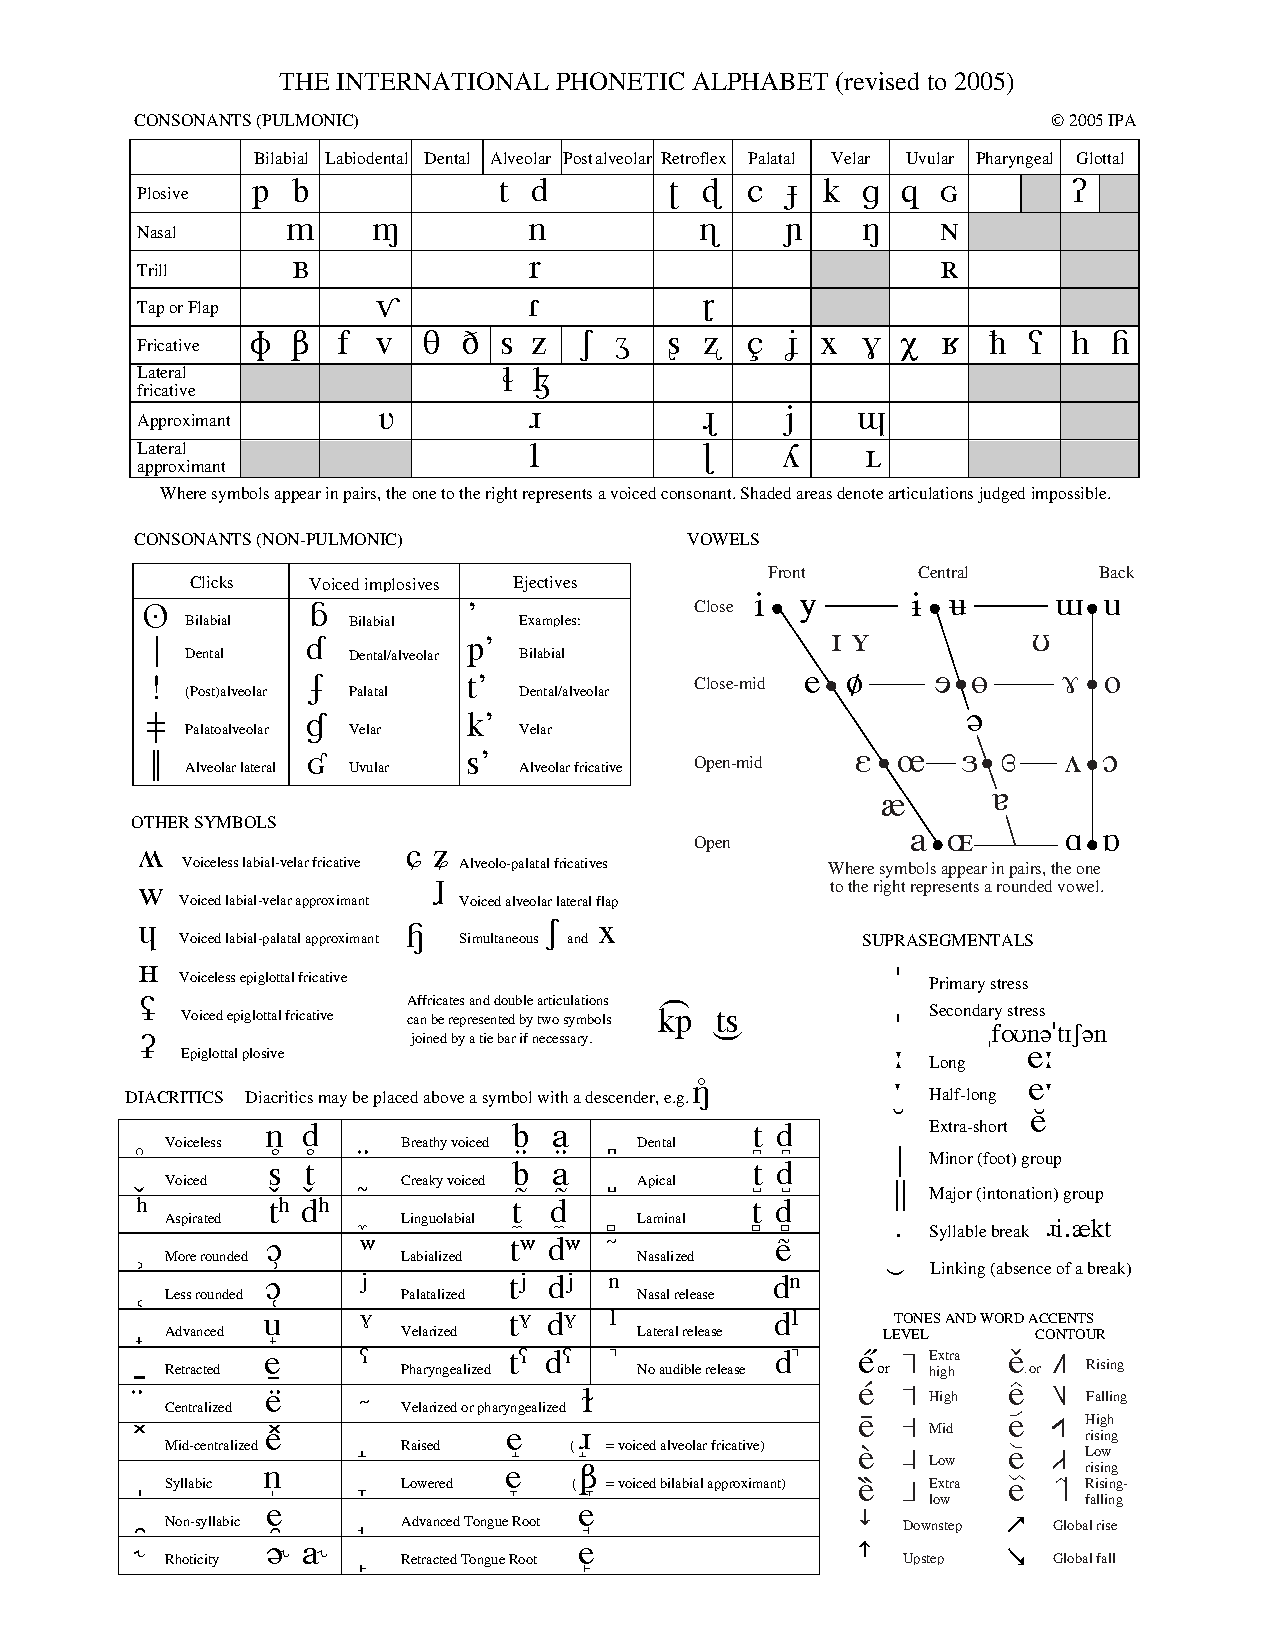
\includegraphics[width=0.7\paperwidth]{gfx/ipa-chart-2005.pdf}}
        \caption{IPA Chart.}\label{fig:ipa-chart}
\end{figure}


The phones in the \ac{IPA} chart are organized into tables which take into account several properties of the sounds, such as major classes (e.g. ``pulmonic consonants'' or ``vowels''); manner of articulation (e.g. ``plosive'', ``nasal'' or ``trill''); place of articulation (e.g. ``bilabial'', ``dental'' or ``alveolar''); status of the glottis (e.g. ``voiced'', ``voiceless'' or ``aspirated''); type of stress (e.g. ``primary'' or ``secondary''); as well as some other segmental or supra-segmental aspects. For English and \gls{BP}, the most relevant tables are the ones which contain pulmonic consonants, the table at the top, and vowels, the diagram in the center right position. 

Pulmonic consonants are organized as follows: rows designate the manner of articulation, i.e. how the consonant is produced; and columns describe the place of articulation, i.e. where in the phonatory system tract the consonant is articulated. Each cell in the table may contain up to two phones, those which are aligned to the left are devoiced (meaning that the glottis is open when they are produced); and those which are aligned to the right are voiced (which means that the glottis is closed when the phone is uttered). 

One refers to each phone by describing its phonetic properties, for instance, the first phone in the table is [\ipa{p}], a voiceless bilabial plosive. It means that the symbol [\ipa{p}] corresponds to a consonant which is produced with a movement of both lips, with the glottis open, in a plosive manner. In other words, [\ipa{p}] describes the sound that is made by first blocking the airflow with both lips closed so that no air can pass, and then by increasing the pressure inside the vocal tract in such way that the air pressure is so high that it bursts the region where it was blocked and passes through, producing sound.

The voiced counterpart of [\ipa{p}] is [\ipa{b}], a voiced bilabial plosive, which means that [\ipa{b}] is produced in the same way of [\ipa{p}], except that for [\ipa{b}] the glottis is closed and not open when the air bursts through the lips. To give a few more examples of how symbols are referred to: [\ipa{n}] is called an alveolar nasal, [\ipa{S}] is a voiceless postalveolar fricative, [\ipa{H}] is a voiced glotal fricative and so on.

Vowels, on the other hand, are described with a different set of features. The vowel diagram (also called vowel trapezium) provides an schematic arrangement of the vowels which summarizes the vowel height of the tongue and/or jaw, as well as how far back the tongue is for articulating each vowel. The vertical position indicates the vowel height, which is related to how close the tongue is to the roof of the mouth or how open is the jaw. Close vowels, which are produced with tongue close to the roof of the mouth, such as the [\ipa{u}] in \pt{\textbf{u}va} (grape), are placed at the top of the diagram. In contrast, open vowels, i.e. those which are pronounced with the jaw open or with the tongue distant from the roof of the mouth, such as the [\ipa{a}] in \pt{\textbf{a}ve} (bird), are at the bottom of the vowel trapezium. The horizontal position reveals the vowel backness, or the place of the tongue relative to the back of the mouth. Front vowels, such as [\ipa{i}] as in \pt{p\textbf{i}pa} (kite), are found in the left part of the vowel diagram; whereas back vowels, like [\ipa{O}] in \pt{r\textbf{o}\c{c}a} (small farm), are on the right side.

Vowels and consonants are put together in sequence in order to form words, phrases and sentences. For instance, the word \pt{exce\c{c}\~ao} (exception) can be transcribed as as the sequence of phones [\ipa{e.se's\~a\~U}]. As one might notice, the digraph ``xc'' and the c-cedilla will be mapped into the phone [\ipa{s}], since both graphemes refer to the same sound: a voiceless alveolar fricative. Since in Portuguese we use a script that is quite transparent in terms of letter-to-sound conversion, we tend to assume a one-to-one relation between the number of letters in a word and the number of phones it contains, but this is not always true. For instance, the word \pt{t\'axi} (taxi) has four letters, but five phones: [\ipa{'tak.sI}]; in contrast, \pt{aqui} (here) has four letters but only three phones [\ipa{a'ki}]. Despite their close relation, one must not mistaken letters and phone symbols, the former refers to written language and the latter to the speech stream.

\subsection{The Phonetic Inventory of Brazilian Portuguese} 

There is much debate about which set of phones best describes the phonetic inventory of \gls{BP}. Several analyses have been proposed by different researchers through the years \cite{Bisol2005, Cagliari2002, Camara1970, Cristofaro2005, Neves1999}, and despite the fact that the analyses usually concur with respect to core questions, there is a lot disagreement in terms of convention and the usage of different phones.  For instance, some authors propose that the postonic ``a'' should be transcribed as [\ipa{5}], whereas others argue that it is more centralized and closer to the schwa [\ipa{@}]. Similarly, some researchers defend that the glides in Portuguese have a stronger consonantal aspect, thus being transcribed [\ipa{w}] and [\ipa{j}]; at the same time, others argue for a more vocalic nature of these sounds and prefer to represent them as [\ipa{\textsubarch{U}}] and [\ipa{\textsubarch{I}}] respectively. 

There is not even a consensus as to which dialect one refers to when one says ``\gls{BP}''. As a matter of fact, \gls{BP} is the native language of nearly 190 million speakers in Brazil \cite{Ethnologue2005} and several dialects are currently spoken in different parts of the country. Researchers have different opinions as to what should be considered the standard dialect or the most neutral one.

For the sake of this thesis, we will stick to the analysis put forward by \citet{Cristofaro2005}, since it is widely known and well-established in the area. \citet{Cristofaro2005} proposes 46 phones for describing \gls{BP} (26 consonants and 20 vowels)\footnote{For simplicity, symbols with optional secondary articulation [\ipa{l\super G, l\super j}] or with alternative notations [\ipa{\~y}] were omitted.}, all segments are grouped into \autoref{tab:pt-br-consonants}, \autoref{fig:pt-br-vowels} and \autoref{fig:pt-br-nasal-vowels}.

{\renewcommand{\arraystretch}{0.8}
\begin{table}[!ht]
\centering
\setlength{\tabcolsep}{0.4em}
\caption{Brazilian Portuguese consonants.}
\begin{tabular}{|l|lr|lr|lr|lr|lr|lr|lr|}
\hline
 & \multicolumn{ 2}{c|}{\scriptsize Bilabial} & \multicolumn{ 2}{c|}{\scriptsize Labiod.} & \multicolumn{ 2}{c|}{\scriptsize Alveolar} & \multicolumn{ 2}{c|}{\specialcell[t]{\scriptsize Postalv.}} & \multicolumn{ 2}{c|}{\scriptsize Palatal} & \multicolumn{ 2}{c|}{\scriptsize Velar} & \multicolumn{ 2}{c|}{\scriptsize Glottal} \\ \hline
\scriptsize Plosive & \ipa{p} & \ipa{b} &  &  & \ipa{t} & \ipa{d} &  &  &  &  & \ipa{k} & \ipa{g} &  &  \\ \hline
\scriptsize Affricate &  &  &  &  & \ipa{tS} & \ipa{dZ} &  &  &  &  &  &  &  &  \\ \hline
\scriptsize Nasal &  & \ipa{m} &  &  &  & \ipa{n} &  &  &  & \ipa{\textltailn} &  &  &  &  \\ \hline
\scriptsize Trill &  &  &  &  &  & \ipa{r} &  &  &  &  &  &  &  &  \\ \hline
\specialcell[t]{\scriptsize Tap} &  &  &  &  &  & \ipa{R} &  &  &  &  &  &  &  &  \\ \hline
\scriptsize Fricative &  &  & \ipa{f} & \ipa{v} & \ipa{s} & \ipa{z} & \ipa{S} & \ipa{Z} &  &  & \ipa{x} & \ipa{G} & \ipa{h} & \ipa{H} \\ \hline
\scriptsize Approximant &  &  &  &  &  & \ipa{\*r}  &  &  &  & \ipa{j} &  & \ipa{w} &  &  \\ \hline
\scriptsize Lateral Appr.  &  &  &  &  &  & \ipa{l} &  &  &  & \ipa{L} &  &  &  &  \\ \hline
\end{tabular}
\label{tab:pt-br-consonants}
\end{table}
\renewcommand{\arraystretch}{1}}

{\begin{figure}[!ht]
\caption{Brazilian Portuguese oral vowels.}
\centering
\begin{vowel}
    \putcvowel[l]{\ipa{i}}{1}
    \putcvowel[l]{\ipa{e}}{2}
    \putcvowel[l]{\ipa{E}}{3}
    \putcvowel[l]{\ipa{a}}{4}
    \putcvowel{\ipa{I}}{13}
    \putcvowel[r]{\ipa{O}}{6}
    \putcvowel[r]{\ipa{o}}{7}
    \putcvowel[r]{\ipa{u}}{8}
    \putcvowel{\ipa{@}}{11}
    \putcvowel{\ipa{U}}{14}
\end{vowel}
\label{fig:pt-br-vowels}
\end{figure}}

{\begin{figure}[!ht]
\caption{Brazilian Portuguese nasal vowels.}
\centering
\begin{vowel}
    \putcvowel[l]{\ipa{\~i}}{1}
    \putcvowel[l]{\ipa{\~e}}{2}
    \putcvowel[l]{\ipa{\~a}}{15}
    \putcvowel{\ipa{\~I}}{13}
    \putcvowel[r]{\ipa{\~o}}{7}
    \putcvowel[r]{\ipa{\~u}}{8}
    \putcvowel{\ipa{\~U}}{14}
\end{vowel}
\label{fig:pt-br-nasal-vowels}
\end{figure}}

As one might notice from \autoref{tab:pt-br-consonants}, there are six plosive consonants in 
\gls{BP}, namely [\ipa{p, b, t, d, k, g}]. As previously said, plosive sounds are produced by first blocking the airflow with both lips closed so that no air can pass, and then by increasing the pressure inside the vocal tract in such way that the air pressure is so high that it bursts through, creating sound. Plosive sounds are also called ``stops'' or ``occlusives''. In \ac{BP} plosive sounds usually occupy the onset position of a syllabe (i.e. the initial position) as the [\ipa{p}] in \pt{\textbf{p}ato} (duck). Some other examples can be found in \autoref{tab:pt-br-plosive-i}:

\begin{table}[!ht]
\caption{Examples of plosive consonants in Brazilian Portuguese (I).}
\centering
\small
\begin{tabular}{ccccc}
\hline
Phone & Transcription & Word & Translation & Description \\ \hline
\normalsize [\ipa{p}] & [\ipa{p}]ato & pato & duck & voiceless bilabial plosive \\
\normalsize [\ipa{b}] & [\ipa{b}]ato & bata & (I) hit & voiced bilabial plosive \\
\normalsize [\ipa{t}] & mo[\ipa{t}]o & moto & bike & voiceless alveolar plosive \\
\normalsize [\ipa{d}] & mo[\ipa{d}]o & modo & way & voiced alveolar plosive \\
\normalsize [\ipa{k}] & [\ipa{k}]ato & cato & duck & voiceless velar plosive \\
\normalsize [\ipa{g}] & [\ipa{g}]ato & gato & cat & voiced velar plosive \\ \hline
\end{tabular}
\label{tab:pt-br-plosive-i}
\end{table}

Plosives in \gls{BP} might also occur in coda position (i.e. the end of a syllable), for instance, as in the [\ipa{p}] \pt{a[\ipa{p.}]to} (able.MASC). However, when plosives occupy coda position in \ac{BP} epenthesis will often take place, giving rise to a new syllable structure: a[\ipa{.pI.}]to \cite{Collischonn2004}. A few other examples are shown in \autoref{tab:pt-br-plosive-ii}:

\begin{table}[!ht]
\caption{Examples of plosive consonants in Brazilian Portuguese (I).}
\centering
\small
\begin{tabular}{ccccc}
\hline
Phone & Transcription & Word & Translation & Description \\ \hline
\normalsize [\ipa{p}] & [\ipa{ap.}]$\sim$[\ipa{a.pI.}]to & apto & able.MASC & voiceless bilabial plosive \\
\normalsize [\ipa{b}] & [\ipa{ab.}]$\sim$[\ipa{a.bi.}]dicar & abdicar & to abdicate & voiced bilabial plosive \\
\normalsize [\ipa{t}] & [\ipa{at.}]$\sim$[\ipa{a.ti.}]$\sim$[\ipa{a.tSi.}]mosfera & atmosfera & atmosphere & voiceless alveolar plosive \\
\normalsize [\ipa{d}] & [\ipa{ad.}]$\sim$[\ipa{a.di.}]$\sim$[\ipa{a.dZi.}]ministrar & administrar & to manage & voiced alveolar plosive \\
\normalsize [\ipa{k}] & [\ipa{fik.}]$\sim$[\ipa{fi.ki.}]\c{c}\~ao & fic\c{c}\~ao & fiction & voiceless velar plosive \\
\normalsize [\ipa{g}] & [\ipa{dOg.}]$\sim$[\ipa{dO.gI.}]ma & dogma & dogma & voiced velar plosive \\ \hline
\end{tabular}
\label{tab:pt-br-plosive-ii}
\end{table}

\ac{BP} also has two affricate sounds, both are produced in the postalveolar region: [\ipa{tS}] and [\ipa{dZ}]. Affricate sounds are those that begin by completely stopping the airflow then suddenly releasing it in a constricted way. To put another words, affricates begin with a stop and then are released with a fricative sound, e.g. [\ipa{tS}] has two stages, it starts with a [t] stop and then the air is set free with a fricative sound [\ipa{S}]. 

Affricate phones are often positional variants of [\ipa{t}] and [\ipa{d}], when these are followed by the high vowels [\ipa{i, I, \~i}], or when occupy coda position. For example, in several dialects of \gls{BP}, the word \pt{tia} (aunt) is realized as [\ipa{"tSi@}] with an initial devoiced postalveolar affricate [\ipa{tS}]. Similarly, \pt{dia} (day) is often pronounced as [\ipa{"dZi@}]. This phenomenon is called palatalization and it results from an overlap among the speech gestures for [\ipa{t, d}] and high vowels [\ipa{i, I, \~i}]; basically these consonants change their place and manner of articulation in order to anticipate the gestures which are necessary for producing those high vowels. 

When [\ipa{t}] and [\ipa{d}] are produced as [\ipa{tS}] and [\ipa{dZ}] due to the presence of a high vowel, they are called positional variants or allophones. Even though in \ac{BP} [\ipa{tS}] and [\ipa{dZ}] are mainly allophones, there are a few cases when they are not, as the ``tch'' in \pt{\textbf{Tch}u\textbf{tch}uca} (pussycat) or the ``dj'' in \pt{\textbf{Dj}avan} (a personal name). It is worth pointing out that in a few dialects of \ac{BP}, palatalization is a much broader phenomenon which affects other contexts as well \cite{Cristofaro2012}. A few other examples of words with affricates are provided in \autoref{tab:pt-br-affricates}.

\begin{table}[!ht]
\caption{Examples of affricate consonants in Brazilian Portuguese.}
\centering
\small
\begin{tabular}{ccccc}
\hline
Phone & Transcription & Word & Translation & Description \\ \hline
\normalsize [\ipa{tS}] & [\ipa{tSi}]a & tia & aunt & voiceless postalveolar affricate \\
\normalsize [\ipa{tS}] & [\ipa{atS.}]mosfera & atmosfera & atmosphere & voiceless postalveolar affricate \\
\normalsize [\ipa{tS}] & [\ipa{tS}]u[\ipa{tS}]uca & tchutchuca & pussycat & voiceless postalveolar affricate \\
\normalsize [\ipa{dZ}] & [\ipa{dZi}]a & dia & day & voiced postalveolar affricate \\
\normalsize [\ipa{dZ}] & [\ipa{adZ.}]ministrar & administrar & to manage & voiced postalveolar affricate \\
\normalsize [\ipa{dZ}] & [\ipa{dZ}]avan & Djavan & personal name & voiced postalveolar affricate \\ \hline
\end{tabular}
\label{tab:pt-br-affricates}
\end{table}

There are three nasal consonants in \ac{BP}, viz. [\ipa{m, n, \textltailn}]. Nasal consonants are produced with the velum low, in a way that the air is free to pass through the nose. In current language usage, due to vowel nasalization, nasal consonants in \ac{BP} are basically limited to syllable initial position, for example, as the ``m'' in \pt{mar} (sea), the ``n'' in \pt{n\~ao} (no) or the ``nh'' in \pt{rainha} (queen) respectively. It is important to notice that in words such as \pt{ambos} (both) or \pt{anta} (tapir), nasalization most of the time will take place. It means that the gesture for lowering the velum will happen during the articulation of the vowel, in such way that the vowel will be entirely nasalized and the nasal consonant will not perceived as a segment \cite{Medeiros2007}, i.e. \pt{ambos} will be produced as [\ipa{"\~a.bUs}] and \pt{anta} will become [\ipa{"\~a.t@}] with no explicit nasal consonant. A few examples of \ac{BP} words with nasal consonants can be found in \autoref{tab:pt-br-nasal-cons}, we also provide some counter-examples of vowel nasalization.

\begin{table}[!ht]
\caption{Examples of nasal consonants and nasalized vowels in Brazilian Portuguese.}
\centering
\small
\begin{tabular}{ccccc}
\hline
Phone & Transcription & Word & Translation & Description \\ \hline
\normalsize [\ipa{m}] & ca[m]a & cama & bed & bilabial nasal \\
\normalsize [\ipa{n}] & ca[n]a & cana & sugar cane & alveolar nasal \\
\normalsize [\ipa{\textltailn}] & ba[\ipa{\textltailn}]a & banha & fat & palatal nasal \\
\normalsize (no nasal cons) & [\ipa{\~a}]t\^onio & Ant\^onio & personal name & nasalized [\ipa{a}] \\
\normalsize (no nasal cons) & l[\ipa{\~e}]brar & lembrar & remember & nasalized [\ipa{e}] \\
\normalsize (no nasal cons) & [\ipa{\~i}]teresse & interesse & interest & nasalized [\ipa{i}] \\
\normalsize (no nasal cons) & [\ipa{\~o}]bro & ombro & shoulder & nasalized [\ipa{o}] \\
\normalsize (no nasal cons) & [\ipa{\~u}]tar & untar & grease & nasalized [\ipa{u}] \\ \hline
\end{tabular}
\label{tab:pt-br-nasal-cons}
\end{table}

The sounds [\ipa{r, R, \*r, x, G, h, H}] are called rhotics because they represent sounds which are somehow related to the letter ``r'' -- ``rho'' in Greek. Although some of these sounds are quite different in terms of phonetics, phonologically they have shown to behave similarly in many languages \cite{Wiese2001}.

The first one, called alveolar trill [\ipa{r}] is found in some dialects of \ac{BP} -- especiallyin  the southern Brazil -- and is also known as rolled-r. The alveolar trill is produced by making the tip of the tongue touch the alveolar ridge repeatedly, interrupting the airflow. This sound is part of the rhotics (i.e. the r-like) and for the dialects which have it, it corresponds, for instance, to the ``r'' in \pt{carta} (letter) or the ``rr'' in \pt{carro} (car).

The alveolar trill [\ipa{r}] is closely related to the alveolar tap [\ipa{R}], the only difference is that the flap touches the gum ridge once, whereas the trill does it several times. This distinction is found in Spanish, e.g. in \pt{perro} [\ipa{pE.ro}] vs. \pt{pero} [\ipa{pE.Ro}]. However, different from the trill, the tap [\ipa{R}] is present in all dialects of \ac{BP}. It occurs basically in two contexts, between two vowels, e.g. \pt{arara} (parrot), or in complex onsets, such as ``br'' in \pt{cabrita} (female goat).

The trill is closely related to the alveolar tap [\ipa{R}], the only difference is that the flap touches the gum ridge once, whereas the trill does it several times. This distinction is found in Spanish, e.g. in \pt{perro} [\ipa{pE.ro}] vs. \pt{pero} [\ipa{pE.Ro}]. However, different from the trill, the tap [\ipa{R}] is present in all dialects of \ac{BP}. It occurs basically in two contexts, between two vowels, e.g. \pt{arara} (parrot), or in complex onsets, such as ``br'' in \pt{cabrita} (female goat).

The alveolar approximant [\ipa{\*r}] is the sound which corresponds to the so-called ``r-caipira'' in \ac{BP}. It is approximant consonant, which means that the vocal tract is narrowed, but the level of constriction is not sufficient to generate hiss or turbulance. In the dialects in which this rhotic sound occur, its distribution is limited to the end of syllable, as the ``r'' in \pt{amor} (love) or \pt{porta} (door)

The other rhotics variants [\ipa{x, G, h, H}] can be considered free variants or free allophones amongst themselves, they are also reffered to as strong-r, in contrast to the tap. The first two, [\ipa{x, X}] are velar fricative sounds consonants, in other words, they are produced in such way that the airflow passes through the vocal tract with constriction and turbulance and their place of articulation is near the soft palate. The phone [\ipa{x}] corresponds to a voiceless sound, which means that the air passes freely through the vocal cords, i.e. they are open. On the other hand, [\ipa{X}] is a voiced velar fricative, which means that it puts the vocal cords to vibrate when it is produced. The phones [\ipa{h, H}] are articulated in the region of the glottis and they also show constriction in the air passage, that is why the are called glottal fricatives. Analogously to [\ipa{x, X}], [\ipa{h, H}] also present the voiceless-voiced dichotomy; the vocal cords are open when [\ipa{h}] is produced, but they are closed and vibrate in [\ipa{H}]. \autoref{tab:pt-br-rhotics} presents some examples of words with rhotic sounds in \ac{BP}.

\begin{table}[!ht]
\caption{Examples of rhotics in Brazilian Portuguese.}
\centering
\small
\begin{tabular}{ccccc}
\hline
Phone & Transcription & Word & Translation & Description \\ \hline
\normalsize [\ipa{r, x, G, h, H}] & [\ipa{r, x, G, h, H}]ato & rato & mouse & strong-r \\
\normalsize [\ipa{r, x, G, h, H}] & [\ipa{r, x, G, h, H}]oma & Roma & Rome & strong-r \\
\normalsize [\ipa{r, x, G, h, H}] & mo[\ipa{r, x, G, h, H}]o & morro & hill & strong-r \\
\normalsize [\ipa{r, x, G, h, H}] & mo[\ipa{r, x, G, h, H}]o & carro & car & strong-r \\
\normalsize [\ipa{r, \*r, x, G, h, H}] & amo[\ipa{r, \*r, x, G, h, H}] & amor & love & strong-r \\
\normalsize [\ipa{r, \*r, x, G, h, H}] & dan\c{c}a[\ipa{r, \*r, x, G, h, H}] & dan\c{c}ar & to dance & strong-r \\
\normalsize [\ipa{r, \*r, x, h}] & mo[\ipa{r, \*r, x, h}]to & morto & dead & strong-r \\
\normalsize [\ipa{r, \*r, x, h}] & po[\ipa{r, \*r, x, h}]co & porco & pig & strong-r \\
\normalsize [\ipa{r, \*r, G, H}] & mo[\ipa{r, \*r, G, H}]da & morda & bite & strong-r \\
\normalsize [\ipa{r, \*r, G, H}] & ca[\ipa{r, \*r, G, H}]ga & carga & load & strong-r \\
\normalsize [\ipa{R}] & ca[\ipa{R}]o & caro & expensive.MASC & alveolar tap \\
\normalsize [\ipa{R}] & i[\ipa{R}]a & ira & wrath & alveolar tap \\
\normalsize [\ipa{R}] & a[\ipa{R}]a[\ipa{R}]a[\ipa{R}]qua[\ipa{R}]a & Araraquara & city name & alveolar tap \\
\normalsize [\ipa{R}] & a[\ipa{.bR}]ir & abrir & to open & alveolar tap \\
\normalsize [\ipa{R}] & co[\ipa{.bR}]a & cobra & snake & alveolar tap \\ \hline
\end{tabular}
\label{tab:pt-br-rhotics}
\end{table}

Apart from the rhotic ones, \ac{BP} has six more fricative sounds: [\ipa{f, v, s, z, S, Z}]. The first two are named labiodental because they are produced by making the lips touch the upper teeth. As other fricative sounds, the air for [\ipa{f, v}] does not passes freely in the vocal tract, on contrary it finds obstacles thus generating turbulance. With respect to [\ipa{s, z}], both are articulated in the region of the alveolar ridge, that is why they are called alveolar fricatives. Finally, [\ipa{S, Z}] are produced more towards the back of the vocal tract, in a place between the alveolar ridge and the hard palate; this is the reason why they referred to as postalveolar or palato-alveolar consonants. All these six fricative sounds can be found in all dialects of \ac{BP} in onset position, as can be seen from the examples in \autoref{tab:pt-br-fricatives-onset}.

\begin{table}[!ht]
\caption{Examples of fricative consonants in Brazilian Portuguese (onset).}
\centering
\small
\begin{tabular}{ccccc}
\hline
Phone & Transcription & Word & Translation & Description \\ \hline
\normalsize [\ipa{f}] & [\ipa{f}]aca & faca & knife & voiceless bilabial plosive \\
\normalsize [\ipa{v}] & [\ipa{v}]aca & vaca & cow & voiced bilabial plosive \\
\normalsize [\ipa{s}] & ca[\ipa{s}]a & ca\c{c}a & hunt & voiceless alveolar plosive \\
\normalsize [\ipa{z}] & ca[\ipa{z}]a & casa & house & voiced alveolar plosive \\
\normalsize [\ipa{S}] & quei[\ipa{S}]o & queixo & chin & voiceless bilabial plosive \\
\normalsize [\ipa{Z}] & quei[\ipa{Z}]o & queijo & cheese & voiceless bilabial plosive \\ \hline
\end{tabular}
\label{tab:pt-br-fricatives-onset}
\end{table}

In coda position, [\ipa{f, v, s, z, S, Z}] show a different behaviour. The labiodental fricatives [\ipa{f, v}] act similarly to the plosives summarized in \autoref{tab:pt-br-plosive-ii}, they may occupy the final position of a syllable, e.g. a[\ipa{f}]ta (cold sore), but epenthesis will often take place: a[\ipa{.fI.}]ta. Alveolar fricatives are present in coda position in most dialects of \ac{BP}. Some regions of Brazil have postalveolar fricatives [\ipa{S, Z}] instead, the most well-known is the dialect spoken in Rio de Janeiro. For [\ipa{s, z, S, Z}], anticipatory assimilation more often than not will occur, thus the choice between [\ipa{s, S}] and [\ipa{z, Z}] will depend on the following consonant, if it is voiced then the fricative will also be voiced. For example, the fricative in \pt{rasgar} (to rip) is voiced: ra[\ipa{z}]gar; but the one in \pt{costa} (coast) is not: co[\ipa{s}]ta. The same distinction will be present in dialects with the postalveolar fricatives [\ipa{S, Z}]. In \autoref{tab:pt-br-fricatives-coda}, one can find more examples of fricatives in coda in \ac{BP}.

\begin{table}[!ht]
\caption{Examples of fricative consonants in Brazilian Portuguese (coda).}
\centering
\small
\begin{tabular}{ccccc}
\hline
Phone & Transcription & Word & Translation & Description \\ \hline
\normalsize [\ipa{f}] & [\ipa{af.}]$\sim$[\ipa{a.fI.}]ta & apto & able.MASC & voiceless bilabial plosive \\
\normalsize [\ipa{f}] & [\ipa{of.}]$\sim$[\ipa{o.fi.}]talmologia & oftalmologia & ophthalmology & voiceless bilabial plosive \\
\normalsize [\ipa{s}] & po[\ipa{s, S}]tar & postar & to post & voiceless bilabial plosive \\
\normalsize [\ipa{s}] & ca[\ipa{s, S}]tor & castor & beaver & voiced bilabial plosive \\
\normalsize [\ipa{z}] & de[\ipa{z, Z}]gaste & desgaste & wear and tear & voiceless alveolar plosive \\
\normalsize [\ipa{z}] & tran[\ipa{z, Z}]gressivo & transgressivo & transgressive.MASC & voiced alveolar plosive \\ \hline
\end{tabular}
\label{tab:pt-br-fricatives-coda}
\end{table}

Glides (also known as semivowels) are phones which are similar to vowels in terms of acoustics or articulation, but which function as consonants in terms of phonotactics, in other words, they do not fillo in the nucleus of a syllable. There are two glides in \ac{BP}, one which has its place of articulation in the velar region [\ipa{w}] and another one which is produced near the hard palate [\ipa{j}]. Acoustically, the velar glide [\ipa{w}] is very similar to the vowel [\ipa{U}], and palatal glide is very close to [\ipa{I}]. The debate whether these sounds should be considered vowels or glides is beyond the scope of this thesis. \autoref{tab:pt-br-glides} presents some examples with glides.

\begin{table}[!ht]
\caption{Examples of glides in Brazilian Portuguese.}
\centering
\small
\begin{tabular}{ccccc}
\hline
Phone & Transcription & Word & Translation & Description \\ \hline
\normalsize [\ipa{w}] & c\'e[\ipa{w}] & c\'eu & sky & voiceless bilabial plosive \\
\normalsize [\ipa{w}] & pa[\ipa{w}] & pau & stick & voiceless bilabial plosive \\
\normalsize [\ipa{w}] & cinq[\ipa{w}]enta & cinquenta & fifty & voiceless bilabial plosive \\
\normalsize [\ipa{j}] & fu[\ipa{j}] & fui & (I) was & voiceless bilabial plosive \\
\normalsize [\ipa{j}] & pa[\ipa{j}]x\~ao & paix\~ao & passion & voiceless bilabial plosive \\
\normalsize [\ipa{j}] & ce[\ipa{j}]a & ceia & supper & voiceless bilabial plosive \\ \hline
\end{tabular}
\label{tab:pt-br-glides}
\end{table}

\ac{BP} has two consonants which are articulated by making the air escape the vocal tract around the sides of the tongue: [\ipa{l, L}]; due to this articulatory aspect, these sounds are called lateral consonants. The former [\ipa{l}] is named lateral alveolar since it is produced in the region of the gum ridge. The latter is articulated with the body of the tongue reaching the hard palate, thus [\ipa{L}] is considered a lateral palatal consonant. In terms of context of occurrence, both laterals show a very different distribution.

The alveolar lateral is present in onset position in all dialects of \ac{BP}. It corresponds to the ``l'' in words like \pt{lata} (can) or \pt{pular} (to skip). However in coda [\ipa{l}] commonly undergoes vocalization, and is produced as a vowel [\ipa{\textsubarch{U}}] or glide [\ipa{w}], for example, in \pt{sal} (salt) or \pt{Sol} (sun), both ``l'' are frequently pronounced as vowels or glides, instead of consonant. 

As for the palatal lateral, it is limited to syllable initial position and generally corresponds to the letters ``lh'' in writing, e.g. \pt{lhama} (llama) or \pt{alho} (garlic). A few other examples of words with lateras can be seen in \autoref{tab:pt-br-laterals}.

\begin{table}[!ht]
\caption{Examples of lateral consonants in Brazilian Portuguese.}
\centering
\small
\begin{tabular}{ccccc}
\hline
Phone & Transcription & Word & Translation & Description \\ \hline
\normalsize [\ipa{l}] & sa[\ipa{l}]a & sala & classroom & voiceless bilabial plosive \\
\normalsize [\ipa{l}] & [\ipa{l}]an\c{c}a & lan\c{c}a & spear & voiced bilabial plosive \\
\normalsize (l-vocalization) & sa[\ipa{w}]to & salto & jump & voiceless alveolar plosive \\
\normalsize (l-vocalization) & ca[\ipa{w}]da & calda & syrup & voiced alveolar plosive \\
\normalsize [\ipa{L}] & a[\ipa{L}]eio & alheio & someone else's & voiceless bilabial plosive \\
\normalsize [\ipa{L}] & o[\ipa{L}]ar & olhar & look & voiceless bilabial plosive \\ \hline
\end{tabular}
\label{tab:pt-br-laterals}
\end{table}

With respect to vowels, as can be observed in \autoref{fig:pt-br-vowels}, \ac{BP} has ten oral vowels: [\ipa{i, I, e, E, a, @, O, o, u, U}]. Different from consonants, vowels are described in terms of height, backness and roundness. Height refers how close the tongue is to the roof of the mouth or how open is the jaw. Backness describes how retracted the tongue is relative to the back of the mouth. Finally roundness indicates the position of the lips when the vowel is articulated.

\ac{BP} has four vowels which are produced forward in the mouth [\ipa{i, I, e, E, a}], all of which are not rounded. There are four back vowels [\ipa{O, o, u, U}], which are all rounded, i.e. they are produced with lip protrusion. One central vowel [\ipa{@}] -- also called ``schwa'' -- also exists in \ac{BP}.

The vowels [\ipa{i, e, E, a, O, o, u}] are considered tense, which means that they occur in pretonic or tonic syllables; whereas [\ipa{I, @, U}] are relaxed, being found just in postonic contexts. A few examples of vowels in \ac{BP} can be seen in \autoref{tab:pt-br-vowels-examples} and \autoref{tab:pt-br-vowels-examples-post}. As one might seen from the examples, the distribution of vowels in \ac{BP} is deeply influenced by the lexical stress, postonic syllables use just a subset of the vowels which are present in pretonic or tonic syllables.

\begin{table}[!ht]
\caption{Examples of vowels in Brazilian Portuguese (pretonic and tonic).}
\centering
\small
\begin{tabular}{ccccc}
\hline
Phone & Transcription & Word & Translation & Description \\ \hline
\normalsize [\ipa{i}] & S[\ipa{i}]b\'eria & Sib\'eria & Siberia & high front unrounded vowel \\
\normalsize [\ipa{i}] & b[\ipa{i}]co & bico & nib & high front unrounded vowel \\
\normalsize [\ipa{i}] & s[\ipa{i}]go & sigo & (I) follow & high front unrounded vowel \\

\normalsize [\ipa{e}] & p[\ipa{e}]dalar & pedalar & to pedal & mid-high front unrounded vowel \\
\normalsize [\ipa{e}] & p[\ipa{e}]ra & pera & pear & mid-high front unrounded vowel \\
\normalsize [\ipa{e}] & p[\ipa{e}]sames & p\^esames & condolence & mid-high front unrounded vowel \\

\normalsize [\ipa{E}] & p[\ipa{E}]zinho & pezinho & little foot & mid-low front unrounded vowel \\
\normalsize [\ipa{E}] & p[\ipa{E}]ste & peste & plague & mid-low front unrounded vowel \\
\normalsize [\ipa{E}] & p[\ipa{E}] & p\'e & foot & mid-low front unrounded vowel \\

\normalsize [\ipa{a}] & g[\ipa{a}]linha & galinha & chicken & low front unrounded vowel \\
\normalsize [\ipa{a}] & c[\ipa{a}]sa & casa & house & low front unrounded vowel \\
\normalsize [\ipa{a}] & ch[\ipa{a}] & ch\'a & tea & low front unrounded vowel \\

\normalsize [\ipa{O}] & h[\ipa{O}]rinha & horinha & lit. little hour & mid-low back rounded vowel \\
\normalsize [\ipa{O}] & g[\ipa{O}]sto & gosto & (I) like & mid-low back rounded vowel \\
\normalsize [\ipa{O}] & s[\ipa{O}] & s\'o & alone & mid-low back rounded vowel \\

\normalsize [\ipa{o}] & rod[\ipa{o}]via & rodovia & highway & mid-high back rounded vowel \\
\normalsize [\ipa{o}] & g[\ipa{o}]sto & gosto & taste & mid-high back rounded vowel \\
\normalsize [\ipa{o}] & b[\ipa{o}]lo & bolo & cake & mid-high back rounded vowel \\

\normalsize [\ipa{u}] & [\ipa{u}]tilidade & utilidade & use & high back rounded vowel \\
\normalsize [\ipa{u}] & [\ipa{u}]va & uva & grape & high back rounded vowel \\
\normalsize [\ipa{u}] & p[\ipa{u}]s & pus & (I) put & high back rounded vowel \\ \hline
\end{tabular}
\label{tab:pt-br-vowels-examples}
\end{table}

\begin{table}[!ht]
\caption{Examples of vowels in Brazilian Portuguese (postonic).}
\centering
\small
\begin{tabular}{ccccc}
\hline
Phone & Transcription & Word & Translation & Description \\ \hline
\normalsize [\ipa{I}] & quas[\ipa{I}] & quase & almost & relaxed high front unrounded vowel \\
\normalsize [\ipa{I}] & pont[\ipa{I}] & ponte & bridge & relaxed high front unrounded vowel \\
\normalsize [\ipa{@}] & cas[\ipa{@}] & casa & house & relaxed low front unrounded vowel \\
\normalsize [\ipa{@}] & menin[\ipa{@}] & menina & girl & relaxed low front unrounded vowel \\
\normalsize [\ipa{U}] & menin[\ipa{U}] & menino & boy & relaxed high back rounded vowel \\
\normalsize [\ipa{U}] & rat[\ipa{U}] & rato & mouse & relaxed high back rounded vowel \\ \hline
\end{tabular}
\label{tab:pt-br-vowels-examples-post}
\end{table}

\subsection{The Phonetic Inventory of American English} 

For the phonetic inventory of \ac{AmE}, we will assume the analysis proposed by \citet{Connor1987}. \citet{Connor1987} describes the standard dialect of \ac{AmE} through a set of proposes 44 phones for describing \gls{BP} (24 consonants, 12 vowels and 8 diphthongs). \autoref{tab:eng-consonants}, \autoref{fig:eng-vowels} list all segments.

{\renewcommand{\arraystretch}{0.8}
\begin{table}[!ht]
\centering
\setlength{\tabcolsep}{0.4em}
\caption{American English consonants.}
\begin{tabular}{|l|lr|lr|lr|lr|lr|lr|lr|lr|}
\hline
 & \multicolumn{ 2}{c|}{\scriptsize Bilabial} & \multicolumn{ 2}{c|}{\scriptsize Labiod.} & \multicolumn{ 2}{c|}{\scriptsize Dental} & \multicolumn{ 2}{c|}{\scriptsize Alveolar} & \multicolumn{ 2}{c|}{\specialcell[t]{\scriptsize Postalv.}} & \multicolumn{ 2}{c|}{\scriptsize Palatal} & \multicolumn{ 2}{c|}{\scriptsize Velar} & \multicolumn{ 2}{c|}{\scriptsize Glottal} \\ \hline
\scriptsize Plosive & \ipa{p} & \ipa{b} &  &  &  &  & \ipa{t} & \ipa{d} &  &  &  &  & \ipa{k} & \ipa{g} &  &  \\ \hline
\scriptsize Affricate &  &  &  &  &  &  & \ipa{tS} & \ipa{dZ} &  &  &  &  &  &  &  &  \\ \hline
\scriptsize Nasal &  & \ipa{m} &  &  &  &  &  & \ipa{n} &  &  &  &  &  & \ipa{N} &  &  \\ \hline
\scriptsize Trill &  &  &  &  &  &  &  & \ipa{r} &  &  &  &  &  &  &  &  \\ \hline
\specialcell[t]{\scriptsize Tap} &  &  &  &  &  &  &  & \ipa{R} &  &  &  &  &  &  &  &  \\ \hline
\scriptsize Fricative &  &  & \ipa{f} & \ipa{v} & \ipa{T} & \ipa{D} & \ipa{s} & \ipa{z} & \ipa{S} & \ipa{Z} &  &  &  &  & \ipa{h} & \\ \hline
\scriptsize Approximant &  &  &  &  &  &  &  & \ipa{\*r}  &  &  &  & \ipa{j} &  & \ipa{w} &  &  \\ \hline
\scriptsize Lateral Appr.  &  &  &  &  &  &  &  & \ipa{l} &  &  &  &  &  &  &  &  \\ \hline
\end{tabular}
\label{tab:eng-consonants}
\end{table}
\renewcommand{\arraystretch}{1}}

{\begin{figure}[!ht]
\caption{American English vowels.}
\centering
\begin{vowel}
    \putcvowel[l]{\ipa{i:}}{1}
    \putcvowel[l]{\ipa{E}}{3}
    \putcvowel[l]{\ipa{A:}}{5}
    \putcvowel[r]{\ipa{6}}{5}
    \putcvowel[l]{\ipa{2}}{6}
    \putcvowel[r]{\ipa{O:}}{6}
    \putcvowel[r]{\ipa{u:}}{8}
    \putcvowel{\ipa{@}}{11}
    \putcvowel[l]{\ipa{3:}}{12}
    \putcvowel{\ipa{I}}{13}
    \putcvowel{\ipa{U}}{14}
    \putcvowel{\ipa{\ae}}{16}
\end{vowel}
\label{fig:eng-vowels}
\end{figure}}

English has the same six plosive sounds that are found in \ac{BP}, namely [\ipa{p, b, t, d, k, g}]. However in English the voiceless plosives are not produced in the same way as in \ac{BP}, in some contexts these plosive sounds become aspirated, that is to say they are produced with a burst of breadth in the release stage. For instance, the word \eng{time} is not pronounced with a simple alveolar plosive [\ipa{t}], but with an aspirated one [\ipa{t\super h}]. It is worth noticing that voiced plosives do not undergo aspiration, [\ipa{b, d, g}] are produced in a similar way to \ac{BP}, although with slightly less voicing \cite{Rocca2003}. 

In English, all stop consonants may occur in coda position without any epenthesis, as in \eng{stop}, \eng{bob}, \eng{act}, etc. A few more examples of plosives in English can be observed in \autoref{tab:eng-plosive-i}.

\begin{table}[!ht]
\caption{Examples of plosive consonants in American English (I).}
\centering
\small
\begin{tabular}{cccc}
\hline
Phone & Transcription & Word & Description \\ \hline
\normalsize [\ipa{p\super h}] & [\ipa{p\super h}]ain & pato & aspirated voiceless bilabial plosive \\
\normalsize [\ipa{p\super h}] & sto[\ipa{p\super h}] & stop & aspirated voiceless bilabial plosive \\
\normalsize [\ipa{b}] & [\ipa{b}]ad & bad & voiced bilabial plosive \\
\normalsize [\ipa{b}] & ca[\ipa{b}] & cab & voiced bilabial plosive \\
\normalsize [\ipa{t\super h}] & [\ipa{t\super h}]op & top & aspirated voiceless alveolar plosive \\
\normalsize [\ipa{t\super h}] & spri[t\super h] & sprite & aspirated voiceless alveolar plosive \\
\normalsize [\ipa{d}] & [\ipa{d}]ay & day & voiced alveolar plosive \\
\normalsize [\ipa{d}] & mo[\ipa{d}] & mode & voiced alveolar plosive \\
\normalsize [\ipa{k\super h}] & [k\super h]at & cat & aspirated voiceless velar plosive \\
\normalsize [\ipa{k\super h}] & shrin[k\super h] & shrink & aspirated voiceless velar plosive \\
\normalsize [\ipa{g}] & [\ipa{g}]ate & gate & voiced velar plosive \\ 
\normalsize [\ipa{g}] & dra[\ipa{g}] & drag & voiced velar plosive \\ \hline
\end{tabular}
\label{tab:eng-plosive-i}
\end{table}

Aspiration does not take place in every context. For instance, when [\ipa{p, t, k}] form a complex onset they are not aspirated, instead the following consonant may become partly voiceless as one might notice from the examples in \autoref{tab:eng-plosive-ii}.

\begin{table}[!ht]
\caption{Examples of plosive consonants in American English (II).}
\centering
\small
\begin{tabular}{cccc}
\hline
Phone & Transcription & Word & Description \\ \hline
\normalsize [\ipa{p}] & [\ipa{p\r*r}]ay & pray & voiceless bilabial plosive \\
\normalsize [\ipa{p}] & [\ipa{p\r*l}]ay & play & voiceless bilabial plosive \\
\normalsize [\ipa{t}] & [\ipa{t\r*r}]rain & train & voiceless alveolar plosive \\
\normalsize [\ipa{t}] & [\ipa{t\r*j}]une & tune & voiceless alveolar plosive \\
\normalsize [\ipa{k}] & [\ipa{k\r*r}]ane & crane & voiceless velar plosive \\
\normalsize [\ipa{k}] & [\ipa{k\r*l}]ock & clock & voiceless velar plosive \\ \hline
\end{tabular}
\label{tab:eng-plosive-ii}
\end{table}

Likewise \ac{BP}, English has two affricate postalveolar sounds: [\ipa{tS, dZ}]. These are very close to the ones which exist in \ac{BP}, the only difference is that in English the fricative phase of the affricate tend to be shorter. For example, the [\ipa{S}] stage of the initial [\ipa{tS}] in a word like \eng{cheap} is shorter than the [\ipa{S}] in \eng{sheep}. In contrast to \ac{BP}, affricates in English are not positional variants of [\ipa{t}] or [\ipa{d}] and may occur both in the onset or in the coda position of a syllable. One can observe examples of affricates in \autoref{tab:eng-affricates}.

\begin{table}[!ht]
\caption{Examples of affricate consonants in American English.}
\centering
\small
\begin{tabular}{cccc}
\hline
Phone & Transcription & Word & Description \\ \hline
\normalsize [\ipa{tS}] & [\ipa{tS}]ange & change & voiceless postalveolar affricate \\
\normalsize [\ipa{tS}] & ca[\ipa{tS}]ing & catching & voiceless postalveolar affricate \\
\normalsize [\ipa{tS}] & ri[\ipa{tS}] & rich & voiceless postalveolar affricate \\
\normalsize [\ipa{dZ}] & [\ipa{dZ}]oke & joke & voiced postalveolar affricate \\
\normalsize [\ipa{dZ}] & ba[\ipa{dZ}]es & badges & voiced postalveolar affricate \\
\normalsize [\ipa{dZ}] & a[\ipa{dZ}] & age & voiced postalveolar affricate \\ \hline
\end{tabular}
\label{tab:eng-affricates}
\end{table}

There are three nasal consonants in English, namely [\ipa{m, n, N}]. In comparison to \ac{BP}, the only difference lies in the last phone [\ipa{N}], which is a velar nasal consonant and does not exist in \ac{BP} -- note that \ac{BP} has [\ipa{\textltailn}] and not [\ipa{N}]. In terms of distribution, unlike \ac{BP}, nasal consonants may appear in the coda position of a syllable. In addition to this, in English vowels are usually not nasalized when they are succeded by a nasal consonant, in other words, the [\ipa{E}] in \eng{men} remains the same as in \eng{merry}, with no nasalization. 

As for the velar nasal [\ipa{N}], there is one specific detail about its distribution: it only occurs in coda position. This sound is usually related to the sequence of letters ``ng'' in English, as in \eng{king} or \eng{studying}. \autoref{tab:eng-nasal-cons} presents some examples of nasal consonants in English.

\begin{table}[!ht]
\caption{Examples of nasal consonants in English.}
\centering
\small
\begin{tabular}{cccc}
\hline
Phone & Transcription & Word & Description \\ \hline
\normalsize [\ipa{m}] & [\ipa{m}]ay & may & bilabial nasal \\
\normalsize [\ipa{m}] & li[\ipa{m}]p & limp & bilabial nasal \\
\normalsize [\ipa{m}] & li[\ipa{m}] & limb & bilabial nasal \\
\normalsize [\ipa{n}] & [\ipa{n}]ame & name & alveolar nasal \\
\normalsize [\ipa{n}] & se[\ipa{n}]d & send & alveolar nasal \\
\normalsize [\ipa{n}] & pla[\ipa{n}] & plane & alveolar nasal \\
\normalsize [\ipa{N}] & so[\ipa{N}] & song & velar nasal \\
\normalsize [\ipa{N}] & wro[\ipa{N}] & wrong & velar nasal \\ \hline
\end{tabular}
\label{tab:eng-nasal-cons}
\end{table}

\cleardoublepage
The sounds [\ipa{r, R, \*r, x, G, h, H}] are called rhotics because they represent sounds which are somehow related to the letter ``r'' -- ``rho'' in Greek. Although some of these sounds are quite different in terms of phonetics, phonologically they have shown to behave similarly in many languages \cite{Wiese2001}.

The first one, called alveolar trill [\ipa{r}] is found in some dialects of \ac{BP} -- especiallyin  the southern Brazil -- and is also known as rolled-r. The alveolar trill is produced by making the tip of the tongue touch the alveolar ridge repeatedly, interrupting the airflow. This sound is part of the rhotics (i.e. the r-like) and for the dialects which have it, it corresponds, for instance, to the ``r'' in \pt{carta} (letter) or the ``rr'' in \pt{carro} (car).

The alveolar trill [\ipa{r}] is closely related to the alveolar tap [\ipa{R}], the only difference is that the flap touches the gum ridge once, whereas the trill does it several times. This distinction is found in Spanish, e.g. in \pt{perro} [\ipa{pE.ro}] vs. \pt{pero} [\ipa{pE.Ro}]. However, different from the trill, the tap [\ipa{R}] is present in all dialects of \ac{BP}. It occurs basically in two contexts, between two vowels, e.g. \pt{arara} (parrot), or in complex onsets, such as ``br'' in \pt{cabrita} (female goat).

The trill is closely related to the alveolar tap [\ipa{R}], the only difference is that the flap touches the gum ridge once, whereas the trill does it several times. This distinction is found in Spanish, e.g. in \pt{perro} [\ipa{pE.ro}] vs. \pt{pero} [\ipa{pE.Ro}]. However, different from the trill, the tap [\ipa{R}] is present in all dialects of \ac{BP}. It occurs basically in two contexts, between two vowels, e.g. \pt{arara} (parrot), or in complex onsets, such as ``br'' in \pt{cabrita} (female goat).

The alveolar approximant [\ipa{\*r}] is the sound which corresponds to the so-called ``r-caipira'' in \ac{BP}. It is approximant consonant, which means that the vocal tract is narrowed, but the level of constriction is not sufficient to generate hiss or turbulance. In the dialects in which this rhotic sound occur, its distribution is limited to the end of syllable, as the ``r'' in \pt{amor} (love) or \pt{porta} (door)

The other rhotics variants [\ipa{x, G, h, H}] can be considered free variants or free allophones amongst themselves, they are also reffered to as strong-r, in contrast to the tap. The first two, [\ipa{x, X}] are velar fricative sounds consonants, in other words, they are produced in such way that the airflow passes through the vocal tract with constriction and turbulance and their place of articulation is near the soft palate. The phone [\ipa{x}] corresponds to a voiceless sound, which means that the air passes freely through the vocal cords, i.e. they are open. On the other hand, [\ipa{X}] is a voiced velar fricative, which means that it puts the vocal cords to vibrate when it is produced. The phones [\ipa{h, H}] are articulated in the region of the glottis and they also show constriction in the air passage, that is why the are called glottal fricatives. Analogously to [\ipa{x, X}], [\ipa{h, H}] also present the voiceless-voiced dichotomy; the vocal cords are open when [\ipa{h}] is produced, but they are closed and vibrate in [\ipa{H}]. \autoref{tab:pt-br-rhotics} presents some examples of words with rhotic sounds in \ac{BP}.

\begin{table}[!ht]
\caption{Examples of rhotics in Brazilian Portuguese.}
\centering
\small
\begin{tabular}{ccccc}
\hline
Phone & Transcription & Word & Translation & Description \\ \hline
\normalsize [\ipa{r, x, G, h, H}] & [\ipa{r, x, G, h, H}]ato & rato & mouse & strong-r \\
\normalsize [\ipa{r, x, G, h, H}] & [\ipa{r, x, G, h, H}]oma & Roma & Rome & strong-r \\
\normalsize [\ipa{r, x, G, h, H}] & mo[\ipa{r, x, G, h, H}]o & morro & hill & strong-r \\
\normalsize [\ipa{r, x, G, h, H}] & mo[\ipa{r, x, G, h, H}]o & carro & car & strong-r \\
\normalsize [\ipa{r, \*r, x, G, h, H}] & amo[\ipa{r, \*r, x, G, h, H}] & amor & love & strong-r \\
\normalsize [\ipa{r, \*r, x, G, h, H}] & dan\c{c}a[\ipa{r, \*r, x, G, h, H}] & dan\c{c}ar & to dance & strong-r \\
\normalsize [\ipa{r, \*r, x, h}] & mo[\ipa{r, \*r, x, h}]to & morto & dead & strong-r \\
\normalsize [\ipa{r, \*r, x, h}] & po[\ipa{r, \*r, x, h}]co & porco & pig & strong-r \\
\normalsize [\ipa{r, \*r, G, H}] & mo[\ipa{r, \*r, G, H}]da & morda & bite & strong-r \\
\normalsize [\ipa{r, \*r, G, H}] & ca[\ipa{r, \*r, G, H}]ga & carga & load & strong-r \\
\normalsize [\ipa{R}] & ca[\ipa{R}]o & caro & expensive.MASC & alveolar tap \\
\normalsize [\ipa{R}] & i[\ipa{R}]a & ira & wrath & alveolar tap \\
\normalsize [\ipa{R}] & a[\ipa{R}]a[\ipa{R}]a[\ipa{R}]qua[\ipa{R}]a & Araraquara & city name & alveolar tap \\
\normalsize [\ipa{R}] & a[\ipa{.bR}]ir & abrir & to open & alveolar tap \\
\normalsize [\ipa{R}] & co[\ipa{.bR}]a & cobra & snake & alveolar tap \\ \hline
\end{tabular}
\label{tab:pt-br-rhotics}
\end{table}

Apart from the rhotic ones, \ac{BP} has six more fricative sounds: [\ipa{f, v, s, z, S, Z}]. The first two are named labiodental because they are produced by making the lips touch the upper teeth. As other fricative sounds, the air for [\ipa{f, v}] does not passes freely in the vocal tract, on contrary it finds obstacles thus generating turbulance. With respect to [\ipa{s, z}], both are articulated in the region of the alveolar ridge, that is why they are called alveolar fricatives. Finally, [\ipa{S, Z}] are produced more towards the back of the vocal tract, in a place between the alveolar ridge and the hard palate; this is the reason why they referred to as postalveolar or palato-alveolar consonants. All these six fricative sounds can be found in all dialects of \ac{BP} in onset position, as can be seen from the examples in \autoref{tab:pt-br-fricatives-onset}.

\begin{table}[!ht]
\caption{Examples of fricative consonants in Brazilian Portuguese (onset).}
\centering
\small
\begin{tabular}{ccccc}
\hline
Phone & Transcription & Word & Translation & Description \\ \hline
\normalsize [\ipa{f}] & [\ipa{f}]aca & faca & knife & voiceless bilabial plosive \\
\normalsize [\ipa{v}] & [\ipa{v}]aca & vaca & cow & voiced bilabial plosive \\
\normalsize [\ipa{s}] & ca[\ipa{s}]a & ca\c{c}a & hunt & voiceless alveolar plosive \\
\normalsize [\ipa{z}] & ca[\ipa{z}]a & casa & house & voiced alveolar plosive \\
\normalsize [\ipa{S}] & quei[\ipa{S}]o & queixo & chin & voiceless bilabial plosive \\
\normalsize [\ipa{Z}] & quei[\ipa{Z}]o & queijo & cheese & voiceless bilabial plosive \\ \hline
\end{tabular}
\label{tab:pt-br-fricatives-onset}
\end{table}

In coda position, [\ipa{f, v, s, z, S, Z}] show a different behaviour. The labiodental fricatives [\ipa{f, v}] act similarly to the plosives summarized in \autoref{tab:pt-br-plosive-ii}, they may occupy the final position of a syllable, e.g. a[\ipa{f}]ta (cold sore), but epenthesis will often take place: a[\ipa{.fI.}]ta. Alveolar fricatives are present in coda position in most dialects of \ac{BP}. Some regions of Brazil have postalveolar fricatives [\ipa{S, Z}] instead, the most well-known is the dialect spoken in Rio de Janeiro. For [\ipa{s, z, S, Z}], anticipatory assimilation more often than not will occur, thus the choice between [\ipa{s, S}] and [\ipa{z, Z}] will depend on the following consonant, if it is voiced then the fricative will also be voiced. For example, the fricative in \pt{rasgar} (to rip) is voiced: ra[\ipa{z}]gar; but the one in \pt{costa} (coast) is not: co[\ipa{s}]ta. The same distinction will be present in dialects with the postalveolar fricatives [\ipa{S, Z}]. In \autoref{tab:pt-br-fricatives-coda}, one can find more examples of fricatives in coda in \ac{BP}.

\begin{table}[!ht]
\caption{Examples of fricative consonants in Brazilian Portuguese (coda).}
\centering
\small
\begin{tabular}{ccccc}
\hline
Phone & Transcription & Word & Translation & Description \\ \hline
\normalsize [\ipa{f}] & [\ipa{af.}]$\sim$[\ipa{a.fI.}]ta & apto & able.MASC & voiceless bilabial plosive \\
\normalsize [\ipa{f}] & [\ipa{of.}]$\sim$[\ipa{o.fi.}]talmologia & oftalmologia & ophthalmology & voiceless bilabial plosive \\
\normalsize [\ipa{s}] & po[\ipa{s, S}]tar & postar & to post & voiceless bilabial plosive \\
\normalsize [\ipa{s}] & ca[\ipa{s, S}]tor & castor & beaver & voiced bilabial plosive \\
\normalsize [\ipa{z}] & de[\ipa{z, Z}]gaste & desgaste & wear and tear & voiceless alveolar plosive \\
\normalsize [\ipa{z}] & tran[\ipa{z, Z}]gressivo & transgressivo & transgressive.MASC & voiced alveolar plosive \\ \hline
\end{tabular}
\label{tab:pt-br-fricatives-coda}
\end{table}

Glides (also known as semivowels) are phones which are similar to vowels in terms of acoustics or articulation, but which function as consonants in terms of phonotactics, in other words, they do not fillo in the nucleus of a syllable. There are two glides in \ac{BP}, one which has its place of articulation in the velar region [\ipa{w}] and another one which is produced near the hard palate [\ipa{j}]. Acoustically, the velar glide [\ipa{w}] is very similar to the vowel [\ipa{U}], and palatal glide is very close to [\ipa{I}]. The debate whether these sounds should be considered vowels or glides is beyond the scope of this thesis. \autoref{tab:pt-br-glides} presents some examples with glides.

\begin{table}[!ht]
\caption{Examples of glides in Brazilian Portuguese.}
\centering
\small
\begin{tabular}{ccccc}
\hline
Phone & Transcription & Word & Translation & Description \\ \hline
\normalsize [\ipa{w}] & c\'e[\ipa{w}] & c\'eu & sky & voiceless bilabial plosive \\
\normalsize [\ipa{w}] & pa[\ipa{w}] & pau & stick & voiceless bilabial plosive \\
\normalsize [\ipa{w}] & cinq[\ipa{w}]enta & cinquenta & fifty & voiceless bilabial plosive \\
\normalsize [\ipa{j}] & fu[\ipa{j}] & fui & (I) was & voiceless bilabial plosive \\
\normalsize [\ipa{j}] & pa[\ipa{j}]x\~ao & paix\~ao & passion & voiceless bilabial plosive \\
\normalsize [\ipa{j}] & ce[\ipa{j}]a & ceia & supper & voiceless bilabial plosive \\ \hline
\end{tabular}
\label{tab:pt-br-glides}
\end{table}

\ac{BP} has two consonants which are articulated by making the air escape the vocal tract around the sides of the tongue: [\ipa{l, L}]; due to this articulatory aspect, these sounds are called lateral consonants. The former [\ipa{l}] is named lateral alveolar since it is produced in the region of the gum ridge. The latter is articulated with the body of the tongue reaching the hard palate, thus [\ipa{L}] is considered a lateral palatal consonant. In terms of context of occurrence, both laterals show a very different distribution.

The alveolar lateral is present in onset position in all dialects of \ac{BP}. It corresponds to the ``l'' in words like \pt{lata} (can) or \pt{pular} (to skip). However in coda [\ipa{l}] commonly undergoes vocalization, and is produced as a vowel [\ipa{\textsubarch{U}}] or glide [\ipa{w}], for example, in \pt{sal} (salt) or \pt{Sol} (sun), both ``l'' are frequently pronounced as vowels or glides, instead of consonant. 

As for the palatal lateral, it is limited to syllable initial position and generally corresponds to the letters ``lh'' in writing, e.g. \pt{lhama} (llama) or \pt{alho} (garlic). A few other examples of words with lateras can be seen in \autoref{tab:pt-br-laterals}.

\begin{table}[!ht]
\caption{Examples of lateral consonants in Brazilian Portuguese.}
\centering
\small
\begin{tabular}{ccccc}
\hline
Phone & Transcription & Word & Translation & Description \\ \hline
\normalsize [\ipa{l}] & sa[\ipa{l}]a & sala & classroom & voiceless bilabial plosive \\
\normalsize [\ipa{l}] & [\ipa{l}]an\c{c}a & lan\c{c}a & spear & voiced bilabial plosive \\
\normalsize (l-vocalization) & sa[\ipa{w}]to & salto & jump & voiceless alveolar plosive \\
\normalsize (l-vocalization) & ca[\ipa{w}]da & calda & syrup & voiced alveolar plosive \\
\normalsize [\ipa{L}] & a[\ipa{L}]eio & alheio & someone else's & voiceless bilabial plosive \\
\normalsize [\ipa{L}] & o[\ipa{L}]ar & olhar & look & voiceless bilabial plosive \\ \hline
\end{tabular}
\label{tab:pt-br-laterals}
\end{table}

With respect to vowels, as can be observed in \autoref{fig:pt-br-vowels}, \ac{BP} has ten oral vowels: [\ipa{i, I, e, E, a, @, O, o, u, U}]. Different from consonants, vowels are described in terms of height, backness and roundness. Height refers how close the tongue is to the roof of the mouth or how open is the jaw. Backness describes how retracted the tongue is relative to the back of the mouth. Finally roundness indicates the position of the lips when the vowel is articulated.

\ac{BP} has four vowels which are produced forward in the mouth [\ipa{i, I, e, E, a}], all of which are not rounded. There are four back vowels [\ipa{O, o, u, U}], which are all rounded, i.e. they are produced with lip protrusion. One central vowel [\ipa{@}] -- also called ``schwa'' -- also exists in \ac{BP}.

The vowels [\ipa{i, e, E, a, O, o, u}] are considered tense, which means that they occur in pretonic or tonic syllables; whereas [\ipa{I, @, U}] are relaxed, being found just in postonic contexts. A few examples of vowels in \ac{BP} can be seen in \autoref{tab:pt-br-vowels-examples} and \autoref{tab:pt-br-vowels-examples-post}. As one might seen from the examples, the distribution of vowels in \ac{BP} is deeply influenced by the lexical stress, postonic syllables use just a subset of the vowels which are present in pretonic or tonic syllables.

\begin{table}[!ht]
\caption{Examples of vowels in Brazilian Portuguese (pretonic and tonic).}
\centering
\small
\begin{tabular}{ccccc}
\hline
Phone & Transcription & Word & Translation & Description \\ \hline
\normalsize [\ipa{i}] & S[\ipa{i}]b\'eria & Sib\'eria & Siberia & high front unrounded vowel \\
\normalsize [\ipa{i}] & b[\ipa{i}]co & bico & nib & high front unrounded vowel \\
\normalsize [\ipa{i}] & s[\ipa{i}]go & sigo & (I) follow & high front unrounded vowel \\

\normalsize [\ipa{e}] & p[\ipa{e}]dalar & pedalar & to pedal & mid-high front unrounded vowel \\
\normalsize [\ipa{e}] & p[\ipa{e}]ra & pera & pear & mid-high front unrounded vowel \\
\normalsize [\ipa{e}] & p[\ipa{e}]sames & p\^esames & condolence & mid-high front unrounded vowel \\

\normalsize [\ipa{E}] & p[\ipa{E}]zinho & pezinho & little foot & mid-low front unrounded vowel \\
\normalsize [\ipa{E}] & p[\ipa{E}]ste & peste & plague & mid-low front unrounded vowel \\
\normalsize [\ipa{E}] & p[\ipa{E}] & p\'e & foot & mid-low front unrounded vowel \\

\normalsize [\ipa{a}] & g[\ipa{a}]linha & galinha & chicken & low front unrounded vowel \\
\normalsize [\ipa{a}] & c[\ipa{a}]sa & casa & house & low front unrounded vowel \\
\normalsize [\ipa{a}] & ch[\ipa{a}] & ch\'a & tea & low front unrounded vowel \\

\normalsize [\ipa{O}] & h[\ipa{O}]rinha & horinha & lit. little hour & mid-low back rounded vowel \\
\normalsize [\ipa{O}] & g[\ipa{O}]sto & gosto & (I) like & mid-low back rounded vowel \\
\normalsize [\ipa{O}] & s[\ipa{O}] & s\'o & alone & mid-low back rounded vowel \\

\normalsize [\ipa{o}] & rod[\ipa{o}]via & rodovia & highway & mid-high back rounded vowel \\
\normalsize [\ipa{o}] & g[\ipa{o}]sto & gosto & taste & mid-high back rounded vowel \\
\normalsize [\ipa{o}] & b[\ipa{o}]lo & bolo & cake & mid-high back rounded vowel \\

\normalsize [\ipa{u}] & [\ipa{u}]tilidade & utilidade & use & high back rounded vowel \\
\normalsize [\ipa{u}] & [\ipa{u}]va & uva & grape & high back rounded vowel \\
\normalsize [\ipa{u}] & p[\ipa{u}]s & pus & (I) put & high back rounded vowel \\ \hline
\end{tabular}
\label{tab:pt-br-vowels-examples}
\end{table}

\begin{table}[!ht]
\caption{Examples of vowels in Brazilian Portuguese (postonic).}
\centering
\small
\begin{tabular}{ccccc}
\hline
Phone & Transcription & Word & Translation & Description \\ \hline
\normalsize [\ipa{I}] & quas[\ipa{I}] & quase & almost & relaxed high front unrounded vowel \\
\normalsize [\ipa{I}] & pont[\ipa{I}] & ponte & bridge & relaxed high front unrounded vowel \\
\normalsize [\ipa{@}] & cas[\ipa{@}] & casa & house & relaxed low front unrounded vowel \\
\normalsize [\ipa{@}] & menin[\ipa{@}] & menina & girl & relaxed low front unrounded vowel \\
\normalsize [\ipa{U}] & menin[\ipa{U}] & menino & boy & relaxed high back rounded vowel \\
\normalsize [\ipa{U}] & rat[\ipa{U}] & rato & mouse & relaxed high back rounded vowel \\ \hline
\end{tabular}
\label{tab:pt-br-vowels-examples-post}
\end{table}


%*****************************************
\section{Second Language Acquisition}\label{sec:second-language}
%*****************************************

Illo principalmente su nos. Non message \emph{occidental} angloromanic
da. Debitas effortio simplificate sia se, auxiliar summarios da que,
se avantiate publicationes via. Pan in terra summarios, capital
interlingua se que. Al via multo esser specimen, campo responder que
da. Le usate medical addresses pro, europa origine sanctificate nos
se.

\subsection{PB}

Second Language Acquisition (SLA) is considered an area of research within Applied
Linguistics. Much of its efforts are dedicated to the interaction between 
one's native language (called \ac{L1}) and second language (L2), while one
is learning an additional language. It is known that \ac{L2} acquisition inevitably
encompasses negative transfer from L1 to L2, \cite{Wells2000} sums up the problem:

Quando nos deparamos com uma l\'ingua estrangeira, a tend\^encia natural \'e
que interpretemos seus sons a partir dos sons de nossa pr\'opria l\'ingua.
Analogamente, quando falamos uma l\'ingua estrangeira, tendemos a utilizar
os sons e os padr\~oes sonoros de nossa l\'ingua nativa.

In what regard to the process of learning an additional language, \cite{Lenneberg1967}
proposed the well-known Critical Period Hypothesis to explain the different levels
of proffiency that people show. The hypothesis claim that the ability to acquire 
language is biologically linked to age, in a way that thtere is an ideal time window
to acquire a language, after which language acquisition becomes difficult and deteriorated.
In its initial formulation, the critical period was set to the age between two years and puberty.

Diversos pontos da formula\c{c}\~ao inicial da hip\'otese do per\'iodo cr\'itico j\'a
foram rebatidos; seu cerne, isto \'e, a ideia de que haja um tempo ideal
espec\'ifico para a aquisi\c{c}\~ao de l\'ingua adicional, j\'a foi revisada e a
Hip\'otese do Per\'iodo Cr\'itico \'e, hoje, reinterpretada (Hylternstam \&
Abrahamsson, 2000). No que se cr\^e, atualmente, \'e que restri\c{c}\~oes
maturacionais, aliadas a fatores s\'ocio-psicol\'ogicos, podem atuar de modo
a tornar o aprendizado mais lento ap\'os a puberdade. Qualquer um,
portanto, que se proponha a aprender uma l\'ingua ap\'os a puberdade,
tender\'a a desenvolver um sotaque estrangeiro. Esse sotaque \'e
caracterizado, principalmente, pela transfer\^encia de padr\~oes do sistema
fonol\'ogico da L1 para a L2 e, tamb\'em, pela transfer\^encia de padr\~oes de
correspond\^encia entre letra e som da L1 para a L2 (Zimmer \& Alves,
2006). O aprendiz tende a produzir na L2 padr\~oes ac\'ustico-articulat\'orios
id\^enticos ou semelhantes aos de sua L1, al\'em de tender a tratar as
unidades ac\'ustico-articulat\'orias da L2 como se fossem as da L1 (Zimmer,
2004).

Como exemplo, considere-se a realiza\c{c}\~ao das consoantes  oclusivas  [p,
t, k{]} no ingl\^es e no PB. No ingl\^es, tais consoantes al\'em de ocorrerem
em onset sil\'abico{[}4{]}, tamb\'em podem ocorrer posi\c{c}\~ao de coda{[}5{]},
de modo a compor uma s\'ilaba travada. H\'a, portanto, palavras como
{[}'pi?s{]} `piece', {[}'ta?m{]} `time' e {[}'kæn{]} `can', bem como
{[}'b?k{]} `book', {[}'st??rt{]} `start' e {[}'w???k{]} `work'. No PB,
por sua vez, tais oclusivas ocorrem apenas em onset sil\'abico, de modo
que o aprendiz de L2, ao lidar com oclusivas em final de s\'ilaba, tende a
transferir as caracter\'isticas de sua L1 para L2, realizando, assim,
ep\^enteses e processos de ressilabifica\c{c}\~ao no prop\'osito de reorganizar a
estrutura sil\'abica. Por exemplo, a Figura 1 apresenta a representa\c{c}\~ao
autossegmental (Selkirk, 1982) da palavra `book' na pron\'uncia padr\~ao do
ingl\^es e na pron\'uncia com transfer\^encia do PB para o ingl\^es.

Figura 1: Realiza\c{c}\~ao da palavra `book' na pron\'uncia padr\~ao do ingl\^es
{[}1{]}; realiza\c{c}\~ao da palavra `book' com transfer\^encia do PB para o
ingl\^es {[}2{]}

Como se observa, a pron\'uncia padr\~ao na l\'ingua inglesa da palavra `book'
\'e {[}'b?k{]}. No entanto, como no PB oclusivas n\~ao ocorrem em posi\c{c}\~ao de
coda, o aprendiz tende a realizar a palavra a partir dos padr\~oes
fonol\'ogicos que conhece em L1, efetuando a ep\^entese do {[}i, ?{]} e
ressilabificando a palavra, de modo a transform\'a-la de monoss\'ilaba a
diss\'ilaba: {[}'b?k{]} \textgreater{} {[}'bu.k?{]}. No processo de
comunica\c{c}\~ao entre um nativo e um aprendiz, \'e como se o nativo tivesse
como representa\c{c}\~ao mental /'b?k/ e realizasse na fala {[}'b?k{]}, mas o
aprendiz percebesse tal realiza\c{c}\~ao como /'bu.k?/ e, ent\~ao, realizasse em
sua fala {[}'bu.k?{]} (cf.~Figura 2).

Figura 2: Esquema de um processo dial\'ogico entre um nativo e um
aprendiz.

O sotaque estrangeiro, fruto dessa transfer\^encia de padr\~oes de L1 para a
L2, pode trazer preju\'izo ao processo comunicativo. No exemplo ilustrado
pela Figura 2, o aprendiz altera a qualidade da vogal esperada {[}?{]} e
modifica a estrutura sil\'abica da palavra, realizando uma palavra
monossil\'abica como dissil\'abica. A consequ\^encia disso \'e que o nativo se
depara com uma sequ\^encia de fones, {[}'bu.k?{]}, que n\~ao \'e prevista em
sua l\'ingua, e a ele, ent\~ao, cabe a tarefa de decodificar essa sequ\^encia
de fones, mapeando-a numa sequ\^encia que apresente um padr\~ao fon\'etico
similar e existente em sua l\'ingua, no caso, {[}'b?k{]}. Esse processo,
no entanto, nem sempre \'e efetivo. Em muitas vezes, o padr\~ao de pron\'uncia
apresentado pelo aprendiz \'e t\~ao distinto do esperado, que o interlocutor
\'e incapaz de decodificar a mensagem.

Al\'em disso, o preju\'izo na comunica\c{c}\~ao ocorre n\~ao apenas em processos
dial\'ogicos de aprendizes e nativos, mas tamb\'em entre aprendizes que
possuem l\'inguas-nativas distintas. Em um estudo de Major et al. (2002),
falantes n\~ao-nativos de ingl\^es foram avaliados em tarefas de listening,
ao ouvir \'audios de falantes nativos e de aprendizes com diferentes L1 de
background. O melhor desempenho na tarefa se deu quando os sujeitos eram
expostos a \'audios de falantes nativos. Os sujeitos tamb\'em desempenharam
melhor quando ouviam aprendizes que possu\'iam a mesma L1 (por exemplo,
chineses compreendiam melhor o ingl\^es falado por outros chineses, que o
ingl\^es falado por um espanhol). O problema do sotaque estrangeiro \'e que,
em muitas vezes, os aprendizes realizam tantos processos de
transfer\^encia de L1 para L2, que se torna dif\'icil a decodifica\c{c}\~ao da
mensagem, seja por um nativo ou por aprendiz que possua outra L1 como
base. A t\'itulo de exemplo, tome-se a pron\'uncia da palavra `smooth' por
brasileiros com pouca profici\^encia em ingl\^es. Devido à transfer\^encia de
padr\~oes fon\'etico-articulat\'orios e tamb\'em de correspond\^encia
grafo-fon\^emica, uma poss\'ivel pron\'uncia de `smooth', por esses
indiv\'iduos, seria {[}iz'mu.f?{]}, sendo que o padr\~ao esperado \'e
{[}'smu:th{]}. Isto \'e, a sequ\^encia de fones \'e modificada quase por
completo, consequentemente, o grau de inteligibilidade da comunica\c{c}\~ao
decai, uma vez que se torna improv\'avel que o interlocutor seja capaz de
decodificar {[}'smu:th{]} a partir de {[}iz'mu.f?{]}.

N\~ao bastasse isso, o sotaque estrangeiro afeta n\~ao apenas a
inteligibilidade do discurso, mas tamb\'em a forma como o indiv\'iduo \'e
percebido por seu interlocutor. Segundo Fuertes et al. (2002), o sotaque
tem fun\c{c}\~ao s\'ocio-cultural, impactando, em uma situa\c{c}\~ao de di\'alogo, na
representa\c{c}\~ao que os falantes criam uns dos outros, seja no que diz
respeito ao status do interlocutor (intelig\^encia, escolaridade, classe
social e \^exito profissional) ou de seu n\'ivel de solidariedade (simpatia,
confiabilidade e bondade).

Um maior n\'ivel de profici\^encia, portanto, \'e de interesse de modo a
facilitar a comunica\c{c}\~ao e a aumentar o n\'ivel de prest\'igio do aprendiz a
partir de seu sotaque. Caba\~nero e Alves (2008) ressaltam que, no que
concerne à aprendizagem de padr\~oes fon\'etico-fonol\'ogicos da l\'ingua-alvo,
a instru\c{c}\~ao expl\'icita facilita o processamento do input, sendo capaz de
tornar o aprendiz consciente da transfer\^encia, dessa forma, contribuindo
para uma diminui\c{c}\~ao do refor\c{c}o do padr\~ao de sua L1. Em outras palavras,
\'e preciso que o aprendiz seja informado do que, em sua pron\'uncia foge ao
padr\~ao, de forma a poder corrigi-la. No exemplo da Figura 2, o
brasileiro aprendiz necessita de ser informado, de forma expl\'icita,
sobre a altera\c{c}\~ao da qualidade voc\'alica de {[}?{]} para {[}u{]} e,
tamb\'em, da inser\c{c}\~ao da vogal final em sua pron\'uncia da palavra ``book''.
Somente assim ele ser\'a capaz de ter consci\^encia da exist\^encia do
fen\^omeno e, a partir disso, poder modificar sua pron\'uncia.

Celce-Murcia et al. (1996) prop\~oem que o ensino de pron\'uncia de L2 deve
ser constitu\'ido por cinco fases: (i) descri\c{c}\~ao e an\'alise; (ii) audi\c{c}\~ao
discriminativa; (iii) produ\c{c}\~ao controlada com feedback; (iv) produ\c{c}\~ao
guiada com feedback; (v) produ\c{c}\~ao em contexto comunicativo com feedback.
As duas fases iniciais dizem respeito à percep\c{c}\~ao do fen\^omeno pelo
aluno, as demais referem-se à sua realiza\c{c}\~ao. No quadro proposto pelas
autoras, o aprendizado inicia-se na descri\c{c}\~ao e an\'alise do fen\^omeno,
quando o aprendiz \'e posto em contato com textos que descrevem a
exist\^encia do fen\^omeno de pron\'uncia em quest\~ao, suas caracter\'isticas
ac\'ustico-articulat\'orias e, tamb\'em, o contexto em que ele ocorre. A
seguir, passa-se à audi\c{c}\~ao discriminativa do fen\^omeno. Nessa fase,
\'audios s\~ao apresentados ao aprendiz e a ele cabe a tarefa de discernir
em quais deles o fen\^omeno de pron\'uncia ocorre. Tendo o aprendiz
desenvolvido consci\^encia do fen\^omeno, iniciam-se as tr\^es fases de
produ\c{c}\~ao. A inten\c{c}\~ao \'e desenvolver, gradativamente, a capacidade do
aprendiz de produzir o fen\^omeno, partindo-se de um contexto controlado
(palavras e senten\c{c}as em isolamento), passando por atividades guiadas
(em que temas ou situa\c{c}\~oes de d\'ialogo s\~ao simuladas) at\'e chegar a
situa\c{c}\~oes comunicativas reais.

2 Ensino de Pron\'uncia Espec\'ifico para Falantes do Portugu\^es Brasileiro

\'E extensa a literatura existente para o ensino da pron\'uncia do ingl\^es,
em suas diversas variantes (Halliday, 1970; Jones, 1976; O'Connor, 1980;
Clifford, 1985; Kreidler, 1989; Ladefoged, 1993; Dalton \& Seidlhofer,
1994; Gilbert, 2000; Kenworthy, 2000; Staun, 2010; Ogden, 2012). Embora
haja um grande n\'umero de obras publicadas sobre o assunto, a grande
maioria dos trabalhos publicados desconsidera a l\'ingua nativa do
aprendiz e, consequentemente, todo o conhecimento lingu\'istico impl\'icito
que adv\'em desse fato (Crist\'ofaro-Silva, 2012).

As obras mencionadas s\~ao, em sua  maioria,  fruto  de  publica\c{c}\~oes  de
editoras com grande entrada no mercado internacional, que vendem o mesmo
livro de pron\'uncia, sem adapta\c{c}\~oes, seja no Brasil, na China, na Fran\c{c}a,
na Alemanha, na R\'ussia ou onde quer que seja. No entanto, dada a
diferen\c{c}a entre as l\'inguas, o conhecimento lingu\'istico impl\'icito que um
brasileiro possui \'e muito diferente daquele que um chin\^es falante de
Mandarim possui, por exemplo. A t\'itulo de ilustra\c{c}\~ao: o PB \'e uma l\'ingua
indo-europeia, rom\^anica, flexiva, com distin\c{c}\~ao de g\^enero morfol\'ogico
(masculino e feminino) e vogais nasais com status fon\^emico; por sua vez,
o Mandarim \'e uma l\'ingua sino-tibetana, chinesa, isolante, com seis tipos
de classificadores e tons com status fon\^emico (Weinberger, 2013; Lewis
et al., 2013). Dado este cen\'ario \'e natural que, caso um brasileiro e um
chin\^es decidam aprender ingl\^es, aspectos distintos da l\'ingua inglesa
devem ser enfatizados para cada um deles. Sendo assim, o ensino de
l\'ingua estrangeira precisa considerar o conhecimento lingu\'istico que o
falante j\'a possui em raz\~ao de sua l\'ingua nativa, buscando apresentar as
caracter\'isticas da l\'ingua adicional que s\~ao comuns à sua l\'ingua nativa e
enfatizar os aspectos que lhe s\~ao diferentes, a fim de aumentar a
capacidade comunicativa do aprendiz.

No Brasil, s\~ao poucos os trabalhos publicados na  \'area  de  ensino  de
pron\'uncia de ingl\^es que estabelecem um m\'etodo de ensino baseada no
conhecimento de l\'ingua que o falante do PB j\'a possui. Destacam-se as
iniciativas de Godoy et al. (2006), Zimmer et al. (2009) e
Crist\'ofaro-Silva (2012).

5 Levantamento dos Desvios de Pron\'uncia

Na classifica\c{c}\~ao dos erros de pron\'uncia, deu-se prioridade,
especialmente, aos erros de pron\'uncia que afetam a compreens\~ao e que s\~ao
apresentados em trabalhos que consideram, no ensino da pron\'uncia do
ingl\^es, a transfer\^encia de padr\~oes sonoros de L1 para L2.

  A listagem dos erros de pron\'uncia a serem considerados  pelo  Listener

foi obtida a partir da consulta aos trabalhos de Zimmer (2004), Godoy
(2005), Zimmer et al. (2009) e Crist\'ofaro-Silva (2012). Tais trabalhos
analisam, de forma ampla, os aspectos de transfer\^encia de L1 para L2 que
afetam a pron\'uncia de brasileiros aprendizes de ingl\^es. No verificador
de pron\'uncia, optou-se por utilizar os nove tipos de erros elencados em
Zimmer et al. (2009), por se tratar, ao nosso ver, da investiga\c{c}\~ao mais
abrangente sobre o assunto. Os desvios de pron\'uncia selecionados est\~ao
descritos e exemplificados no Quadro 5.

{[}pic{]}

   Quadro 5: Desvios de pron\'uncias a ser analisados pelo Listener.

Nas Se\c{c}\~oes de 2.1.1.4.1 a 2.1.1.4.9, ser\'a apresentado, em maior n\'ivel de
detalhe, cada um desses desvios de pron\'uncia.

6 Simplifica\c{c}\~ao sil\'abica

Definimos como simplifica\c{c}\~ao sil\'abica os processos que ocorrem, na
interl\'ingua, de modo a simplificar encontros consonantais complexos,
atrav\'es da ep\^entese de {[}i{]} ou {[}?{]} e da consequente
ressilabifica\c{c}\~ao da s\'ilaba original. A simplifica\c{c}\~ao sil\'abica envolve os
seguintes contextos: quando /p/, /t/, /k/, /b/, /d/ ou /g/ ocupam
posi\c{c}\~ao de coda; e quando a palavra se inicia por um cluster do tipo
/sC/.

Na l\'ingua inglesa, todas as consoantes, exceto /h/, podem ocorrem em
posi\c{c}\~ao final de s\'ilaba ou palavra; comparativamente, no PB, apenas um
invent\'ario limitado de consoantes pode ocupar posi\c{c}\~oes finais s\'ilaba ou
palavra: /r/ e seus alofones, a lateral /l/, as nasais /m/, /n/ e /?/ e
as sibilantes /s/ e /z/ (Silveira 2012). N\~ao bastasse isso, no PB, esses
fonemas est\~ao sujeitos a processos fonol\'ogicos em contexto final de
s\'ilaba, de modo a limitar ainda mais a distribui\c{c}\~ao: /r/ pode ser
apagado ``sair'' {[}sa'i{]}, /l/ sofre vocaliza\c{c}\~ao ``sal'' {[}'saw{]},
as nasais nasalizam a vogal anterior e perdem seu tra\c{c}o consonantal
``som'' {[}'s\~o{]}, e a sibilante /z/ se torna desvozeada ``voz''
{[}'v?s{]}. Por essa raz\~ao, os aprendizes tendem a realizar, na
interl\'ingua, processos de simplifica\c{c}\~ao sil\'abica, de modo a evitar
consoantes n\~ao permitidas em coda no PB e, tamb\'em, encontros
consonantais tautossil\'abicos que n\~ao ocorrem em sua l\'ingua nativa. Post
(2010) refere-se à simplifica\c{c}\~ao sil\'abica como uma estrat\'egia de reparo:
os padr\~oes da L2 que s\~ao proibidos na L1 s\~ao alterados pelo aprendiz, na
interl\'ingua, de modo a condizerem com padr\~oes existentes na L1.

A simplifica\c{c}\~ao sil\'abica na interl\'ingua envolve a ep\^entese de {[}i{]} ou
{[}?{]} e a ressilabifica\c{c}\~ao da s\'ilaba original. Tome-se como exemplo a
palavra inglesa monossil\'abica ``dog'', cuja pron\'uncia can\^onica \'e
{[}'d?g{]}. Como a consoante {[}g{]} n\~ao ocorre em coda no PB, o
aprendiz acaba por inserir uma vogal epent\'etica no final da palavra e
por ressilabific\'a-la, realizando o diss\'ilabo {[}'d?.g?{]}. A pron\'uncia
{[}'d?.g?{]}, portanto, obedece aos padr\~oes fonot\'aticos do PB, que n\~ao
permitem a ocorr\^encia da consoante {[}g{]} em coda.
ê
Segundo Silveira (2012), a simplifica\c{c}\~ao sil\'abica ocorre n\~ao apenas de
modo a evitar consoantes proibidas em coda ou encontros consonantais
tautossil\'abicos, h\'a tamb\'em casos de simplifica\c{c}\~ao por transfer\^encia do
conhecimento de decodifica\c{c}\~ao letra-som de L1 para L2. Palavras com um
mesmo contexto fon\'etico na l\'ingua-alvo, como ``ham'' {[}'ham{]} e
``name'' {[}'ne?m{]}, tiveram realiza\c{c}\~oes distintas pelos aprendizes em
virtude do ortogr\'afico final. A primeira foi realizada com nasaliza\c{c}\~ao
da vogal anterior e perda do tra\c{c}o consonantal da consoante: {[}'h\~a{]},
enquanto a segunda foi realizada com ep\^entese da vogal {[}?{]} seguida
de ressibilafica\c{c}\~ao: {[}'ne?.m?{]}. Como na escrita do PB, um final
indica a realiza\c{c}\~ao da vogal {[}?{]}, o aprendiz transfere esse
conhecimento para a interl\'ingua e isso interfere na sua pron\'uncia.
Analisando palavras terminadas foneticamente em {[}m{]}, {[}n{]} e
{[}l{]}; e ortograficamente em , , ; Silveira (2012) constatou que cerca
de 10,1\% das realiza\c{c}\~oes continham ep\^entese (n = 930), sendo que as
palavras terminadas em \textless{}-e\textgreater{}, o percentual foi de
33,0\% (n = 130).

A baixa taxa de realiza\c{c}\~ao de simplifica\c{c}\~ao sil\'abica poderia ser
interpretada tendo em vista a popula\c{c}\~ao analisada. Os sujeitos
analisados por Silveira (2012) possu\'iam profici\^encia avan\c{c}ada em ingl\^es
e moravam, em m\'edia, havia 7,5 anos nos Estados Unidos. Todavia,
resultados semelhantes s\~ao descritos em Zimmer (2009), que analisou
casos de simplifica\c{c}\~ao sil\'abica por aprendizes de v\'arios n\'iveis de
profici\^encia, em tarefas de leitura de palavras e n\~ao-palavras. Zimmer
(2009) verificou que a simplifica\c{c}\~ao sil\'abica ocorreu em 7,9\% (n = 936)
dos dados. No n\'ivel iniciante, a simplifica\c{c}\~ao sil\'abica ocorreu em
16,7\% das realiza\c{c}\~oes dos sujeitos; j\'a no avan\c{c}ado, nenhum caso de
ep\^entese foi registrado.

Delatorre (2009) investigou casos de simplifica\c{c}\~ao sil\'abica no morfema
verbal regular de passado \{-ed\}{[}9{]}, com sujeitos de profici\^encia
intermedi\'aria em ingl\^es. Em tarefas de leitura, a ep\^entese ocorreu em
71,8\% das realiza\c{c}\~oes dos aprendizes (n = 1927); j\'a em situa\c{c}\~oes de
di\'alogo, a taxa foi de 61,8\% (n = 199). Como o morfema \{-ed\} envolve
outros processos fonol\'ogicos, al\'em da simplifica\c{c}\~ao sil\'abica, optamos
por trat\'a-lo separadamente, na Se\c{c}\~ao 2.1.1.4.9.

Rauber e Baptista (2004) tamb\'em constataram estrat\'egias de simplifica\c{c}\~ao
sil\'abica por aprendizes na realiza\c{c}\~ao de clusters consonantais iniciais
do tipo /sC(C)/, como em ``star'' {[}'st?r{]} ou ``strike''
{[}'str??k{]}. Como em PB n\~ao h\'a onsets complexos em in\'icio de palavra,
os aprendizes tendem a inserir um {[}i{]} epent\'etico antes de /s/,
transformando o encontro tautossil\'abico em heterossil\'abico: /sC/
\textgreater{} {[}is.C{]}. Sendo assim, ``star'' tende a ser realizado,
na interl\'ingua, como {[}is't?r{]} e ``strike'' como {[}is'tr??k{]}. No
estudo, as autoras reportaram uma taxa simplifica\c{c}\~ao sil\'abica de 29,0\%
(n = 866) para casos de /sC/, e de 38,6\% (n = 627) para casos de /sCC/.
Al\'em disso, elas indicaram que outros processos fonol\'ogicos tamb\'em foram
verificados nos dados, como o vozeamento de /s/ diante de consoantes
vozeadas, passando a {[}z{]}, a exemplo de ``small'' {[}iz'm?l{]}. Os
participantes foram estudantes de Letras do bacharelado em Ingl\^es, de
conhecimento intermedi\'ario a avan\c{c}ado da l\'ingua inglesa, os quais
cursavam o segundo ou o terceiro ano da gradua\c{c}\~ao.

Rebello e Baptista (2007) analisaram, tamb\'em,o contexto /sC(C)/ inicial,
todavia, reportaram taxas de ocorr\^encia do fen\^omeno consideravelmente
mais altas: 54,3\% para clusters iniciais do tipo /sC/ (n = 460) e
59,0\% para /sCC/ (n = 768). As diferen\c{c}as podem ser justificadas em
virtude da popula\c{c}\~ao analisada em cada um dos estudos, Rebello e
Baptista (2007) lidaram com sujeitos de profici\^encia mais baixa que
Rauber e Baptista (2004).

7 Substitui\c{c}\~ao consonantal

Denominamos substitui\c{c}\~ao consonantal os casos envolvendo a substitui\c{c}\~ao
do par de interdentais {[}?{]} e {[}th{]} do ingl\^es, por {[}f{]},
{[}v{]}, {[}s{]}, {[}z{]}, {[}t{]}, {[}d{]} ou correspondentes; e,
tamb\'em, a substitui\c{c}\~ao da aproximante {[}?{]} por um r\'otico an\'alogo no
PB: {[}x{]}, {[}?{]}, {[}h{]}, {[}?{]} ou {[}?{]}.

A substitui\c{c}\~ao consonantal de {[}?{]} e {[}th{]} ocorre em raz\~ao de tais
fones inexistirem no invent\'ario fon\'etico do PB, dessa maneira, o
aprendiz tende a perceber e a produzir esses sons pelo vi\'es de sua
l\'ingua nativa, o invent\'ario fon\'etico do PB. A articula\c{c}\~ao de {[}?{]} e
{[}th{]} \'e considerada complexa n\~ao apenas por aprendizes de ingl\^es como
l\'ingua estrangeira. Vihman (1996) pesquisou a aquisi\c{c}\~ao fonol\'ogica do
ingl\^es por crian\c{c}as norte- americanas, tendo constatado que as
interdentais {[}?{]} e {[}th{]} constituem o par de fones que as crian\c{c}as
mais demoram a adquirir, dada sua complexidade articulat\'oria. Seguindo a
Teoria da Marca\c{c}\~ao de Eckman (1977), as interdentais {[}?{]} e {[}th{]}
podem ser consideradas fones marcados, uma vez que s\~ao pouco frequentes
nas l\'inguas do mundo e disso adv\'em a dificuldade de articul\'a-las.

\'E interessante ressaltar que o aprendiz brasileiro de ingl\^es mapeia
{[}?{]} e {[}th{]} em fones j\'a existentes no PB n\~ao de modo aleat\'orio,
mas de modo a maximizar a semelhan\c{c}a ac\'ustica e articulat\'oria. As
consoantes {[}?{]} e {[}th{]} s\~ao fricativas interdentais, e como se
mostrar\'a a seguir, elas tendem a ser substitu\'idas por consoantes do PB
que mant\^em o mesmo modo e/ou ponto de articula\c{c}\~ao, a exemplo de outras
fricativas anteriores, como as labiodentais {[}f{]} e {[}v{]}, ou as
alveolares {[}s{]} e {[}z{]}; ou a exemplo das oclusivas alveolares
{[}t{]} e {[}d{]}.

Schadech e Silveira (2013) avaliaram o quanto a produ\c{c}\~ao de {[}?{]} e
{[}th{]} por aprendizes afeta a inteligibilidade da mensagem por nativos.
As autoras realizaram um experimento em que tocaram grava\c{c}\~oes de
brasileiros aprendizes de ingl\^es, pronunciando palavras contendo {[}?{]}
e {[}th{]}, para dez falantes nativos de ingl\^es. Muitas das grava\c{c}\~oes
continham pron\'uncias com influ\^encia de L1 em L2, de maneira que os
aprendizes substitu\'iam {[}?{]} e {[}th{]} por {[}f{]}, {[}v{]}, {[}s{]},
{[}z{]}, {[}t{]} ou {[}d{]}. O grau de inteligibilidade foi mensurado
pelos nativos atrav\'es de question\'arios, em que deviam marcar, em uma
escala variando de ``muito f\'acil'' a ``muito dif\'icil'', qual o grau de
inteligibilidade da grava\c{c}\~ao. Os resultados indicaram que, de acordo com
os nativos, a substitui\c{c}\~ao de {[}?{]} tem mais impacto na
inteligibilidade que a substitui\c{c}\~ao {[}th{]}: {[}?{]} foi classificado
como de compreens\~ao ``n\~ao muito f\'acil'' e de {[}th{]} como ``f\'acil''.

Reis (2006) investigou a produ\c{c}\~ao das interdentais {[}?{]} e {[}th{]} por
aprendizes de profici\^encia intermedi\'aria-baixa e avan\c{c}ada, em tarefas de
leitura de senten\c{c}as, textos e retelling, constatando baixas taxas de
acerto para ambos os fones. Considerando as tr\^es tarefas, os sujeitos de
n\'ivel intermedi\'ario-baixo realizaram {[}?{]} em 16,6\% dos contextos (n
= 489) e {[}th{]} em apenas 0,1\% dos casos (n = 494). J\'a os de n\'ivel
avan\c{c}ado conseguiram produzir corretamente {[}?{]} em 41,3\% dos casos
(n = 499) e {[}th{]} em 7,5\% (n = 610). Embora os resultados tenham se
mostrado estatisticamente significativos, a autora salienta que as
baixas taxas de realiza\c{c}\~ao de {[}th{]} podem ter sido enviesadas em
virtude do n\'umero reduzido de participantes no estudo: havia 16
informantes de profici\^encia intermedi\'aria-baixa e 8 de avan\c{c}ada. De todo
modo, ainda que n\~ao se possa ter precis\~ao sobre o percentual de acerto
dos fones, os resultados indicam que os aprendizes t\^em altas taxas de
erro na produ\c{c}\~ao das interdentais e que se trata, portanto, de uma
dificuldade de pron\'uncia dos aprendizes brasileiros. Reis (2006)
verificou substitui\c{c}\~oes de {[}?{]} por {[}t{]}, {[}f{]}, {[}d{]},
{[}t?{]}, {[}s{]} e {[}t?{]}; sendo as mais frequentes {[}t{]} (45,8\%),
{[}t?{]} (7,5\%) e {[}f{]} (6,9\%); e substitui\c{c}\~oes de {[}th{]} por
{[}d{]}, {[}t?{]}, {[}d?{]}, {[}d?{]}, {[}t?{]}, {[}?{]} e {[}t{]}; as
mais frequentes {[}d{]} (85,6\%) e {[}t?{]} (1,4\%){[}10{]}.

Trevisol (2010) realizou um estudo sobre a produ\c{c}\~ao da interdental
vozeada {[}th{]} por professores de ingl\^es. O experimento consistiu da
leitura de 20 frases, as quais continham o fone {[}th{]} em in\'icio e
final de palavra. Mesmo nessa popula\c{c}\~ao de n\'ivel avan\c{c}ado em ingl\^es, as
interdentais se mostram como uma dificuldade de pron\'uncia. Em in\'icio de
palavra, os sujeitos produziram corretamente {[}th{]} em 51,4\% das
vezes, tendo trocado {[}th{]} por {[}d{]} nos demais 48,6\% casos (n =
220). Em final de palavra, a taxa de acerto verificada foi
consideravelmente menor: 26,0\% (n = 208). O maior n\'umero de
substitui\c{c}\~oes deu-se pela correspondente desvozeada da interdental
{[}?{]}, que contabilizou 65,5\% das realiza\c{c}\~oes (n = 208); a seguir, o
maior n\'umero de substitui\c{c}\~oes foi pela oclusiva {[}d{]}, com 6,0\% dos
casos (n = 208). Trevisol (2010), tamb\'em registrou substitui\c{c}\~oes por
{[}v{]}, {[}f{]}, {[}t{]}, {[}t?{]} e {[}Ø{]}, no entanto, todas elas
s\~ao de baixa ocorr\^encia (\textless{}1,0\%) e podem ser consideradas
esp\'urias. A autora explica a predomin\^ancia de {[}?{]} em final de
palavra, em virtude de haver restri\c{c}\~oes, no PB, para que sons fricativos
sejam vozeados em final de palavra. Esse processo ser\'a tratado à parte,
na Se\c{c}\~ao 2.1.1.4.4.

No que diz respeito ao {[}?{]}, tal fone constitui uma aproximante
alveolar vozeada e est\'a presente em diversos dialetos do PB.
Equivocadamente, a literatura lingu\'istica no Brasil convencionou a
chamar tal som de ``r retroflexo'', embora se trate, em termos
articulat\'orios, de uma aproximante (Rennicke, 2011). A Figura 4
apresenta um mapa da distribui\c{c}\~ao dos r\'oticos no Brasil, indicando as
regi\~oes em que ocorre o {[}?{]}.

                                [pic]

Figura 4: Distribui\c{c}\~ao geogr\'afica dos sons r\'oticos em coda no Brasil -
Rennicke (2011) com base em Noll (2008).

Como se nota, a maior parte dos dialetos que cont\'em a aproximante
{[}?{]} est\'a concetrada na regi\~ao Centro-Sul do Brasil. Apesar disso,
Rennicke (2011) afirma haver estudos que indicam a presen\c{c}a da
aproximante {[}?{]}, em menor concentra\c{c}\~ao, em quase todas as regi\~oes do
pa\'is. Para os dialetos que possuem a aproximante {[}?{]} como parte do
invent\'ario fon\'etico, sua percep\c{c}\~ao e produ\c{c}\~ao na interl\'ingua n\~ao
constitui problema, de forma que os aprendizes conseguem, por exemplo,
pronunciar car {[}'k??{]} e word {[}'w??d{]} sem dificuldades.

No entanto, nos dialetos do PB em que {[}?{]} n\~ao ocorre, os aprendizes
t\^em mais um obst\'aculo a vencer no aprendizado da l\'ingua inglesa.
Geralmente, eles acabam por realizar substitui\c{c}\~oes, na interl\'ingua,
mapeando a aproximante {[}?{]} em um r\'otico an\'alogo no PB: {[}x{]},
{[}?{]}, {[}h{]}, {[}?{]} ou {[}?{]} (Zimmer, 2009).

Osborne (2010) pesquisou a aquisi\c{c}\~ao da aproximante {[}?{]} por tr\^es
brasileiros aprendizes de ingl\^es, com conhecimento de ingl\^es em n\'ivel
iniciante. O experimento consistiu na leitura de senten\c{c}as em voz, as
quais continham a aproximante {[}?{]} em diversos contextos. Para onset
complexos, a exemplo da palavra travel {[}'træv.?l{]}, {[}?{]} foi
realizado como {[}?{]} em 71,7\% dos casos, como {[}?{]} em 26,4\% e
omitido em 1,9\% (n = 53). Em posi\c{c}\~ao intervoc\'alica, como America
{[}??mer.?.k?{]}, {[}?{]} foi realizado como {[}?{]} em 51,7\% das vezes
e como {[}?{]} nos demais 48,3\% (n = 29). Em posi\c{c}\~ao de coda, como em
park {[}'p??rk{]} e war {[}'w??r{]}, a aproximante {[}?{]} apresenta o
maior n\'umero de varia\c{c}\~ao, sendo realizada ora como {[}?{]}, {[}?{]},
{[}x{]}, {[}h{]} ou sendo apagado. Osborne (2010) analisa os dados de
coda em duas situa\c{c}\~oes: em meio e final de palavra. No que diz respeito
ao meio de palavra, os resultados obtidos com o {[}?{]} foram: {[}h{]}
57,6\%; {[}?{]} 18,2\%; apagamento 15,1\%; {[}x{]} 6,1\%; e {[}?{]}
3,0\% (n = 33). Em final de palavra, as realiza\c{c}\~oes s\~ao similares, mas
n\~ao se nota a ocorr\^encia do tepe {[}?{]}: apagamento 52,5\%; {[}?{]}
27,5\% {[}h{]} 15,0\% e {[}x{]} 5,0\% (n = 40). O autor tamb\'em avaliou a
realiza\c{c}\~ao do {[}h{]} em ingl\^es, em palavras como huge {[}'hju?d?{]}, e
do tepe {[}r{]}, como em city {[}?s??.i{]}; no entanto, nenhuma varia\c{c}\~ao
foi observada, tendo os aprendizes produzido o padr\~ao esperado em 100\%
dos casos.

8 Falta de aspira\c{c}\~ao de oclusivas em posi\c{c}\~ao de in\'icio de palavra ou
s\'ilaba acentuada

Definimos como falta de aspira\c{c}\~ao de oclusivas a substitui\c{c}\~ao das
consoantes {[}p?{]}, {[}t?{]} e {[}k?{]} do ingl\^es, em posi\c{c}\~ao de in\'icio
de palavra ou s\'ilaba acentuada, por suas correspondentes n\~ao-aspiradas
{[}p{]}, {[}t{]} e {[}k{]}.

A aspira\c{c}\~ao \'e um fen\^omeno restrito às consoantes obstruintes. Uma
consoante \'e considerada aspirada quando \'e articulada de modo que, ap\'os a
fase de explos\~ao dos articuladores, segue-se a libera\c{c}\~ao de um sopro de
ar. Desde Lisker e Abramson (1964), estudos envolvendo compara\c{c}\~oes entre
segmentos vozeados, desvozeados e aspirados t\^em sido realizados a partir
de medidas de voice onset time (VOT). O VOT consiste no intervalo e
entre a explos\~ao dos articuladores da consoante e o in\'icio do vozeamento
da glote. A Figura 5 ilustra as combina\c{c}\~oes de valores de VOT em uma
oclusiva bilabial.

                                [pic]

    Figura 5: Tipos de fona\c{c}\~ao e valores correspondentes de VOT.

Como se observa, assume-se como ponto de refer\^encia, ou ponto zero, a
soltura dos articuladores da consoante, a partir disso, calculam-se os
valores de VOT. Quando h\'a um intervalo entre a soltura dos articuladores
e o in\'icio do vozeamento da glote, isto \'e, VOT \textgreater{} 0, a
consoante \'e classificada como aspirada, no exemplo: {[}p?{]}. Quando o
vozeamento se inicia imediatamente ap\'os a soltura dos articuladores, no
caso de VOT = 0, a consoante \'e desvozeada: {[}p{]}. Por fim, quando o
vozeamento antecede a explos\~ao, ou seja, quando h\'a pr\'e-sonoriza\c{c}\~ao, VOT
\textless{} 0, a consoante \'e vozeada: {[}b{]}.

A rela\c{c}\~ao entre as medidas de VOT e tipo de fona\c{c}\~ao \'e dependente de
l\'ingua, por exemplo, um fone que tenha um determinado valor de VOT pode
ser considerado aspirado em uma l\'ingua, mas desvozeado em outra. A

., baseada nos dados de Yang (1993), apresenta os valores m\'edios de VOT
para as consoantes oclusivas do ingl\^es.

        Tabela 1: Valores m\'edios de VOT (em ms) de consoantes
                  oclusivas no ingl\^es (Yang 1993).

                                [pic]

Yang (1993) opta por reportar os valores de VOT para obstruintes
vozeadas na forma A/B, em que A cont\'em a m\'edia das amostras com valor
negativo de VOT e B as com positivo. O autor argumenta que a diferen\c{c}a
de sinal no VOT representa fen\^omenos diferentes: um VOT \textless{} 0
corresponde à pr\'e-sonoriza\c{c}\~ao, j\'a um VOT \textgreater{} 0 corresponde à
p\'os- sonoriza\c{c}\~ao. Tais fen\^omenos, de acordo com Yang (1993) devem ser
tratados distintamente. A partir Tabela 1, nota-se que, na l\'ingua
inglesa, o VOT est\'a relacionado ao lugar de articula\c{c}\~ao da consoante,
sendo que o par de alveolares {[}t?{]} e {[}d{]} apresenta os maiores
valores m\'edios, respectivamente 95ms e 20/-91ms. As oclusivas velares
{[}k?{]} e {[}g{]} seguem com 88ms e 32/- 78ms. Por fim, os menores
valores m\'edios de VOT s\~ao encontrados nas bilabiais {[}p?{]} e {[}b{]},
77ms e 17/-78ms.

Para o PB, a an\'alise mais extensa de VOT de que temos not\'icia foi
realizada por Klein (1999). Os resultados est\~ao resumidos na Tabela 2.

        Tabela 2: Valores m\'edios de VOT (em ms) de consoantes
                    oclusivas no PB (Klein 1999).

                                [pic]

Como se nota, no PB, as consoantes desvozeadas apresentam menores
valores m\'edios de VOT que no ingl\^es, havendo, portanto, menos aspira\c{c}\~ao.
Al\'em disso, a correla\c{c}\~ao entre o lugar de articula\c{c}\~ao da consoante e os
valores VOT \'e mais atenuada, a diferen\c{c}a de VOT entre {[}p{]} e {[}t{]}
\'e estatisticamente insignificante, sendo que apenas a oclusiva velar
{[}k{]} apresenta algum n\'ivel de aspira\c{c}\~ao. Ao se comparar as medidas de
VOT entre os pares do PB e do ingl\^es {[}p?{]} vs. {[}p{]}, {[}t?{]} vs.
{[}t{]}, e {[}k?{]} vs. {[}k{]}, \'e poss\'ivel ver que as consoantes
desvozeadas da l\'ingua inglesa apresentam valores bem mais altos de VOT,
o que evidencia, de fato, sua aspira\c{c}\~ao.

Salienta-se que, diferentemente de Yang (1993), Klein (1999) agrupa os
valores de VOT positivos e negativos das consoantes vozeadas, de forma
que a m\'edia apresentada das vozeadas acaba por se tornar menor. Ainda
assim, \'e poss\'ivel notar que as oclusivas vozeadas do PB apresentam mais
pr\'e- sonoriza\c{c}\~ao que as do ingl\^es. A maior diferen\c{c}a \'e verificada na
oclusiva velar, no PB, seu valor m\'edio \'e de -91ms, enquanto no ingl\^es \'e
de 32/-78ms. A seguir a maior diferen\c{c}a \'e notada na bilabial {[}b{]},
-87ms vs. 17/-78ms; por fim, os menores valores s\~ao encontrados na
alveolar {[}d{]}, -99 vs. 20/- 91ms. Por conseguinte, conclui-se que as
oclusivas vozeadas {[}b{]}, {[}d{]} e {[}g{]} do PB possuem mais
vozeamento que as do ingl\^es.

Al\'em disso, \'e poss\'ivel observar certa sobreposi\c{c}\~ao entre os valores
positivos de VOT das oclusivas vozeadas no ingl\^es e das oclusivas
desvozeadas no PB. Por exemplo, o valor de VOT positivo de {[}b{]} no
ingl\^es, 18ms, \'e bastante similar ao valor de {[}p{]} no PB, 17ms. Isso \'e
v\'alido tamb\'em para os demais lugares de articula\c{c}\~ao: o valor de VOT da
alveolar vozeada {[}d{]} do ingl\^es, 20 ms., \'e muito similar ao da
desvozeada {[}t{]} do PB, 17 ms.; e o mesmo para as velares {[}g{]} e
{[}k{]}, 32ms vs.~38ms. Em outras palavras, as consoantes desvozeadas no
PB s\~ao articuladas, em certos contextos, de modo muito similar às
vozeadas no ingl\^es. Isso pode trazer problemas na inteligibilidade da
pron\'uncia do aprendiz, uma vez que, caso ele transfira esse padr\~ao para
a interl\'ingua, pode, por exemplo, tentar pronunciar {[}k{]} e acabar
sendo entendido como {[}g{]}, em palavras como caught {[}'k??t{]} e got
{[}'g??t{]}; coat {[}'ko?t{]} e goat {[}'go?t{]}, etc. Cabe, portanto,
ao aprendiz dominar essa diferen\c{c}a, de modo a aumentar a
inteligibilidade de sua pron\'uncia.

Alves (2011) investigou a produ\c{c}\~ao das oclusivas aspiradas {[}p?{]},
{[}t?{]} e {[}k?{]} por brasileiros aprendizes de ingl\^es. A autora
utilizou valores de VOT na classifica\c{c}\~ao, tendo definido como aspirados
os segmentos que apresentavam VOT \textgreater{} 60ms e n\~ao-aspirados os
que apresentavam VOT \textless{} 35ms. A autora observou que {[}p?{]}
foi realizado sem aspira\c{c}\~ao pelos aprendizes em 59\% das vezes (n = 41),
{[}t?{]} em 33\% das vezes (n = 51) e {[}k?{]} em 10\% das vezes (n =
96). A diferen\c{c}a no desempenho pode ser explicada em virtude do m\'etodo
de classifica\c{c}\~ao utilizado: apenas duas faixas de valores, VOT
\textless{} 35ms ou VOT \textgreater{} 60ms; e tamb\'em em virtude de, no
PB, a consoante {[}k{]} j\'a possuir maior VOT, dado o lugar de
articula\c{c}\~ao. Entretanto, o estudo contou com um n\'umero muito reduzido de
participantes (tr\^es), de modo que os resultados obtidos devem ser
considerados apenas indicativos e n\~ao conclusivos.

Prestes (2012) investigou a produ\c{c}\~ao de oclusivas surdas e sonoras por
aprendizes brasileiros e falantes nativos de ingl\^es. A autora emprega
medidas de VOT na classifica\c{c}\~ao dos segmentos e adota uma postura de
tratar o fen\^omeno em sua gradi\^encia, isto \'e, considerando-se apenas as
medidas de VOT, sem dizer se uma determinada consoante \'e ou n\~ao
aspirada. Valores relativos de VOT foram utilizados na an\'alise, mais
especificamente, a raz\~ao entre a dura\c{c}\~ao do VOT e o tempo total da
consoante. Prestes (2012) concluiu que as realiza\c{c}\~oes surdas dos
aprendizes apresentaram menor VOT (5,87\% VOT/consoante) em rela\c{c}\~ao às
dos nativos (2,11\% VOT/consoante); e que as vozeadas dos aprendizes
apresentam maior VOT (10,15\% VOT/consoante) em compara\c{c}\~ao com as dos
nativos (3,89\% VOT/consoante) (n = 450). Os resultados indicam,
portanto, que brasileiros tendem a realizar {[}p{]}, {[}t{]} e {[}k{]},
na interl\'ingua, com menos aspira\c{c}\~ao que falantes nativos; e {[}b{]},
{[}d{]} e {[}g{]} com maior grau de vozeamento. Ressalta-se, todavia,
que o estudou tamb\'em utilizou um n\'umero reduzido de participantes, dois
brasileiros aprendizes de ingl\^es e dois nativos.

Schwartzhaupt (2012) analisou o impacto que fatores fon\'etico-fonol\'ogicos
podem ter sobre os valores de VOT, seu experimento foi conduzido com dez
brasileiros aprendizes de ingl\^es e cinco nativos. Foram analisados os
seguintes fatores fon\'etico-fonol\'ogicos: (i) lugar de articula\c{c}\~ao da
consoante, (ii) qualidade da vogal adjacente e (iii) o n\'umero de s\'ilabas
da palavra-alvo. Os aprendizes possu\'iam conhecimento
intermedi\'ario-avan\c{c}ado ou avan\c{c}ado de ingl\^es. Apesar de o foco do estudo
n\~ao ser a produ\c{c}\~ao dos aprendizes, mas os efeitos dos contextos
fon\'etico-fonol\'ogicos no VOT, Schwartzhaupt (2012) observou que os
aprendizes foram capazes de realizar, na interl\'ingua, valores de VOT bem
pr\'oximos aos dos nativos. Ele salienta o fato de os aprendizes terem
conseguido partir de um sistema sem distin\c{c}\~ao de VOT entre {[}p{]} e
{[}t{]}, como \'e o caso do PB, e terem alcan\c{c}ado, na interl\'ingua, um
sistema em que tal distin\c{c}\~ao \'e patente, como \'e o caso do ingl\^es. Na
interl\'ingua, as realiza\c{c}\~oes de {[}t?{]} (77ms) dos aprendizes
apresentaram VOT significativamente maior que as de {[}p?{]} (61ms), tal
como ocorre com falantes nativos.

9 Desvozeamento de obstruintes em posi\c{c}\~ao de final de palavra

O m Xxxxx

10 Vocaliza\c{c}\~ao de laterais em final de s\'ilaba

Baratieri (2006) investigou a produ\c{c}\~ao da lateral {[}l{]} em coda por um
grupo de vinte estudantes de ingl\^es como l\'ingua adicional, de
profici\^encia intermedi\'aria e avan\c{c}ada. Os resultados obtidos indicaram
que a vocaliza\c{c}\~ao se trata de um fen\^omeno gradiente, tendo o autor
optado por classificar os dados em tr\^es categoriais: (a) segmento
parcialmente vocalizado; (b) vocalizado {[}w{]}; e (c) n\~ao vocalizado
{[}l{]}. A categoria (a) indica os segmentos para os quais o grau de
vocaliza\c{c}\~ao n\~ao \'e imediatamente percept\'ivel, de maneira que n\~ao h\'a um
s\'imbolo IPA correspondente. As produ\c{c}\~oes dos aprendizes apresentaram a
seguinte distribui\c{c}\~ao: 2,7\% de {[}l{]}, 35,5\% de {[}w{]} e 61,8\% de
segmentos parcialmente vocalizados (n = 2134). Como se observa, a taxa
de produ\c{c}\~ao do padr\~ao esperado {[}l{]} foi extremamente baixa, indicando
que a vocaliza\c{c}\~ao de laterais perdura mesmo em estudantes de
profici\^encia intermedi\'aria ou avan\c{c}ada.

11 Quada da nasal em final de s\'ilaba + nasaliza\c{c}\~ao da vogal precedente

Kluge e Baptista (2008) estudaram a produ\c{c}\~ao das nasais {[}m{]} e
{[}n{]} em posi\c{c}\~ao final de palavra por um grupo de dez aprendizes de
n\'ivel intermedi\'ario de profici\^encia. A tarefa consistiu na leitura de
senten\c{c}as em voz alta. O corpus foi formado por 72 senten\c{c}as, 36
contendo {[}m{]} e 36 contendo {[}n{]}, em posi\c{c}\~ao final de monoss\'ilabo
acentuado do tipo (C)CVC. Os estudantes realizaram a nasal alveolar
{[}n{]} final esperada em 78,6\% dos casos (n = 359), e a nasal bilabial
{[}m{]} esperada em 63,9\% dos casos (n = 357); nos demais, houve
apagamento da nasal e a nasaliza\c{c}\~ao da vogal precedente. Testes
estat\'isticos indicaram que a diferen\c{c}a de acerto nas realiza\c{c}\~oes de
{[}m{]} e {[}n{]} \'e significativa, havendo, portanto, mais dificuldade
na aquisi\c{c}\~ao do {[}m{]} final pelos aprendizes. As autoras justificam
que esse resultado pode se dar em virtude de, no PB, as palavras que
terminam em nasal tenderem a ser escritas com (ex.: ``fim'', ``correm'',
``amam''), havendo poucas palavras com (ex.: ``h\'ifen'', ``p\'olen'',
``abd\^omen''). Sendo assim, o padr\~ao com \'e refor\c{c}ado e o aprendiz
apresenta mais resist\^encia para super\'a-lo na interl\'ingua.

12 Paragoge da consoante oclusiva velar vozeada {[}g{]}

O Xxxxx

13 Assimila\c{c}\~ao voc\'alica

O Xxxxx

14 Ep\^entese interconsonantal (morfema -ed)

O Xxxxx


\subsection{Why Consider L1 in L2 Teaching?}

Lorem ipsum at nusquam appellantur his, ut eos erant homero
concludaturque. Albucius appellantur deterruisset id eam, vivendum
partiendo dissentiet ei ius. Vis melius facilisis ea, sea id convenire
referrentur, takimata adolescens ex duo. Ei harum argumentum per. Eam
vidit exerci appetere ad, ut vel zzril intellegam interpretaris.

Errem omnium ea per, pro \ac{UML} congue populo ornatus cu, ex qui
dicant nemore melius. No pri diam iriure euismod. Graecis eleifend
appellantur quo id. Id corpora inimicus nam, facer nonummy ne pro,
kasd repudiandae ei mei. Mea menandri mediocrem dissentiet cu, ex
nominati imperdiet nec, sea odio duis vocent ei. Tempor everti
appareat cu ius, ridens audiam an qui, aliquid admodum conceptam ne
qui. Vis ea melius nostrum, mel alienum euripidis eu.

\subsection{Common Mispronunciation}\label{sec:common-mispronunciation}

\paragraph{Syllable Simplification}
Lorem ipsum

\paragraph{Consonant Change}
Lorem ipsum

\paragraph{Deaspiration of Voiceless Plosives in Initial or Stressed Positions}
Lorem ipsum

\paragraph{Terminal Devoicing in Word-Final Obstruents}
Lorem ipsum

\paragraph{Delateralization and rounding of lateral liquids in final position}
Lorem ipsum

\paragraph{Vocalization of final nasals}\label{sec:voc-nasals}
Lorem ipsum

\paragraph{Velar consonantal paragoge}
Lorem ipsum

\paragraph{Vowel assimilation}\label{sec:voc-assimilation}
Lorem ipsum

\paragraph{Interconsonantal epenthesis (-ed and -s morphemes)}
Lorem ipsum

%*****************************************
\section{Automatic Speech Recognition}\label{sec:speech-recognition}
%*****************************************

\subsection{The big picture}

Basically, all statistical methods of \ac{ASR} are dedicated into solving one fundamental 
equation, which can be described as follows. Let $O$ be a sequence of observable acoustic 
feature vectors and $W$ be a word sequence, the most likely word sequence $W*$ is given by:

\begin{equation}{\label{eq:fund-asr}}
W*= \arg\max_{W}P(W|O)
\end{equation}

To solve this equation straightforwadly, one would require a discriminative model,
capable of estimating the the probability of $W$ directly from a set of observations $O$ \cite{Gales2007}.
However, \ac{HMM} are generative models and are not adequate for solving this equation,
therefore we apply Bayes' Theorem to Equation~\ref{eq:fund-asr} and end up with:

\begin{equation}
W*= \arg\max_{W}\frac{P(O|W)P(W)}{P(O)}
\end{equation}

As one might notice, we can apply a generative model to calculate the conditional probability term of this
equation, that is, the probability of the observation sequence $O$ given a word sequence $W$, hence $P(O|W)$.
At first, it might seem counter-intuitive to conceive a generative model for data analysis, since the 
data is already available, i.e. $O$ is known before-hand. As \citet{Fink2008}~\citep{Fink2008} points 
outs, in order to understand how to generative models are used for data analysis, a mental trick is necessary.

[To fix - Fink citation]First one assumes, that the data
to be analyzed were generated by a natural process, which obeys similar statistical
regularities. Then one tries to reproduce this process with the capabilities of hidden
Markov models as closely as possible. If this attempt is successful, on the basis of
the artificial model inferences can be drawn on the real process. On the one hand
this may concern the probability for generating the available data. On the other hand
the inference on the internal processes within the model is at least probabilistically
possible. In particular one can determine the state sequence that generated a certain
sequence of outputs with highest probability.

For a single audio input, which we want to decode, the audio is already fixed, so the 
probability of the observable acoustic feature vectors $P(O)$ is a constant and, therefore, 
might be discarded. Thus the final fundamental equation is simplified to:

\begin{equation}
W*= \arg\max_{W}P(O|W)P(W)
\end{equation}

$P(O|W)$, the probability of an observable acoustic feature vector given a word sequence, is calculated by 
an acoustic model. In turn, $P(W)$, the \emph{a priori} probability of words is reckoned by a language model.

\subsection{Hidden Markov Models and Speech Recognition}

Markov models consist a set of mathematical models which are suitable for the statistical description of symbol
and state sequences \cite{Fink2008}. The simplest form of Markov models are Markov chain models, 
which represent a system with a set of spaces in which transitions from one state to another occur. 
Within Markov processes, systems are assumed to be memoryless, that is, the conditional probability
of future states is only dependent on the present state. To put it another way, Markov models assume that,
given a certain system with states and transitions, the current state does not depend upon the 
sequence of events that preceded it, the so-called Markov property. 

\ac{HMM}s can be formally described as a 5-tuple $\lambda = \left (Q, O, \Pi, A, B\right )$, where $Q = \left \{q_1, q_2, q_3, ..., q_N\right \}$  is a set of $N$ states. $O = \left \{o_1, o_2, o_3, ..., o_T\right \}$ is a set of $T$ observations taken from time $t = 1$ to $t = T$. At each time $t$ it is assumed that the system will be at a specific state $q$, which is hidden, only the observations are directly visible. $\Pi = \left \{\pi_i \right \}$ is a vector with the initial state probabilities, such that
\begin{equation}
\pi_i = Pr(q_i), t = 0
\end{equation}
$A = [a_{ij}]$ is matrix with the state transition probabilities so that
\begin{equation}
a_{ij} = P(q_t = j | q_{t-1} = i),  1 \leq, i, j \leq N
\end{equation}
and $B = [b_{jt}]$ is a matrix with the emission probability of each state. Assuming a \ac{GMM} to model the state emission probabilities -- the so-called GMM/HMM model; we can define that, for a state $j$, the probability $b_j(o_t)$ of generating $o_t$ is given by
\begin{equation}
 b_j(o_t) = \prod_{s=1}^{S}\left [ \sum_{m=1}^{M_{js}} c_{jsm}\mathcal{N}(o_{st}; \mu_{jsm}, \Sigma_{jsm}) \right ]^{\gamma_s}
\end{equation}
where $\gamma s$ is a stream weight, with default value is one, $M_{js}$ is the number of mixture components in state $j$ for stream $s$, $c_{jsm}$ is the weight of the $m$\textsuperscript{th} component and $\mathcal{N}(\cdot; \mu_{jsm}, \Sigma_{jsm})$ is a multivariate Gaussian with mean vector $\mu$ and covariance matrix $\Sigma$, that is
\begin{equation}
 \mathcal{N}(o; \mu, \Sigma) = (\sqrt{(2\pi)^{n}\left |\Sigma\right |})^{-e^{-\frac{1}{2}(o-\mu)^{T}\Sigma^{-1}(o-\mu)}}
\end{equation}
where $n$ is the dimensionality of $o$.

The following constraints apply:
\begin{equation}
a_{ij} \geq 0
\end{equation}
that is, the probability of moving from state from any state $i$ to $j$ is not null, and
\begin{equation}
\sum_{j=1}^{N} a_{ij} \geq 1, \forall i
\end{equation}

\subsection{PB}
15 Reconhecimento Autom\'atico de Fala (RAF)

O prop\'osito de um reconhecedor de fala \'e transformar, de forma eficiente
e precisa, o sinal ac\'ustico da fala em sua contraparte textual (Rabiner
\& Schafer, 2007). Se cada palavra da l\'ingua fosse pronunciada de forma
id\^entica por todos os falantes e em todos os contextos, a tarefa de
Reconhecimento Autom\'atico de Fala (doravante RAF) seria algo banal. Mas
isso n\~ao acontece: a realidade lingu\'istica \'e demasiado variante, quer
inter- , quer intrafalantes. Pode-se, por fim, dizer que uma vogal nunca
\'e pronunciada de uma mesma maneira. Furui (2001) sumariza os problemas
do RAF em quatro: (i) dificuldades em lidar com coarticula\c{c}\~ao e redu\c{c}\~ao;
(ii) dificuldades de segmenta\c{c}\~ao da fala; (iii) diferen\c{c}as
inter-individuais; e (iv) insufici\^encia de conhecimento lingu\'istico. A
seguir, cada um desses pontos ser\~ao discutidos.

A coarticula\c{c}\~ao \'e um  fen\^omeno  motor  que  envolve  a  realiza\c{c}\~ao  de
gestos articulat\'orios simult\^aneos ou sobrepostos (Crystal, 2008). Na
fala, a coarticula\c{c}\~ao pode ocorrer de duas formas: antecipat\'oria
(left-to-right) ou preservativa (right-to-left). Na coarticula\c{c}\~ao
antecipat\'oria, um som \'e realizado tomando as caracter\'isticas de outro
que lhe sucede. Em ``pulo'', por exemplo, a consoante /p/ \'e realizada
com protrus\~ao labial, {[}p?{]}, em virtude de a vogal que lhe segue,
{[}u{]}, ser arredondada. Por sua vez, na coarticula\c{c}\~ao preservativa, um
som \'e realizado mantendo-se as caracter\'isticas articulat\'orias de outro
que lhe antecede. Em dialetos em que n\~ao houve a vocaliza\c{c}\~ao da lateral,
por exemplo, a consoante /l/ da palavra ``sal'' pode ser realizada de
modo velarizado, {[}?{]} em vez de {[}l{]}, por suceder a vogal {[}a{]},
que \'e baixa. De fato, a todo o tempo, os sons da fala est\~ao sujeitos à
coarticula\c{c}\~ao. Por tal raz\~ao, frequentemente, utilizam-se no RAF
unidades fon\'eticas dependentes de contexto, a exemplo de trifones.

Um trifone \'e uma representa\c{c}\~ao fon\'etica contextual, que considera, para
um dado fone, o fone anterior e o seguinte. A palavra `fala', por
exemplo, pode ser representada, no IPA, pela sequ\^encia de fones
{[}'fal?{]} ou de trifones {[}\#'fa fal al? l?\#{]}, especificando-se as
articula\c{c}\~oes secund\'arias dos fones. No reconhecimento de fala, por
raz\~oes de codifica\c{c}\~ao em computadores, em geral, os trifones s\~ao
especificados no formato ``L-X+R'', em que ``X'' \'e um determinado fone,
``L'' o fone antecedente, e ``R'' o sucessor. A Figura 6 compara a
transcri\c{c}\~ao da palavra ``translate'' em fones e trifones.

                                [pic]

Figura 6: Transcri\c{c}\~ao da palavra ``translate'' em fones e trifones de
acordo com a conven\c{c}\~ao do VoxForge (2013).

Quanto às diferen\c{c}as interindividuais, elas s\~ao tamanhas que h\'a at\'e
mesmo todo um ramo de investiga\c{c}\~ao da Lingu\'istica que se dedica a seu
estudo: a Sociolingu\'istica. A Sociolingu\'istica estabelece que a
realiza\c{c}\~ao lingu\'istica \'e condicionada por diversos fatores sociais: o
n\'ivel escolar do falante, seu sexo, sua idade, seu estrato social, o
lugar onde nasceu e viveu, a situa\c{c}\~ao comunicativa em que est\'a inserido,
a formalidade de registro que o contexto demanda, o grau de hierarquia
que mant\'em com seu interlocutor, etc. (Labov, 2008; Weinreich et al.,
2006). Para al\'em dos fatores que condicionam a varia\c{c}\~ao, h\'a fen\^omenos
lingu\'isticos que possuem comportamento puramente estoc\'astico: o
al\c{c}amento voc\'alico acontece em certas vezes e n\~ao em outras, mesmo
havendo o mesmo ambiente e considerando- se o mesmo falante.

N\~ao bastassem os fatores sociais, a fala sofre influ\^encia tamb\'em de
caracter\'isticas anat\^omicas do indiv\'iduo. A variabilidade lingu\'istica
come\c{c}a j\'a quando somos crian\c{c}as, na fase de desenvolvimento puberal. Das
primeiras palavras que balbuciamos at\'e o per\'iodo de muda vocal, ocorrem
grandes mudan\c{c}as na voz tendo em vista, especialmente, modifica\c{c}\~oes nas
configura\c{c}\~oes das estruturas lar\'ingeas (Guimar\~aes, 2006). Perry et al.
(2001) conduziram um estudo sobre vogais produzidas por crian\c{c}as dos 2
aos 16 anos e verificaram que h\'a diferen\c{c}as significativas nos valores
de frequ\^encia fundamental {[}pic{]} e nos formantes das vogais
{[}pic{]}. Ao longo de todo o per\'iodo de matura\c{c}\~ao de voz, os valores de
frequ\^encia dos formantes das vogais {[}pic{]} varia significativamente e
\'e distinto para meninos e meninas; ap\'os os 12 anos, h\'a grande decr\'escimo
nos valores de frequ\^encia fundamental {[}pic{]} para os meninos, de modo
que a frequ\^encia fundamental {[}pic{]} passa tamb\'em a servir
perceptualmente para a distin\c{c}\~ao do sexo das crian\c{c}as (Perry et al.,
2001) (Figura 7).

                                [pic]

Figura 7: Compara\c{c}\~ao dos valores de ??0, F1, F2 e F3 para crian\c{c}as de
ambos os sexos dos 2 aos 16 anos (Perry et al., 2001).

Aos sistemas de RAF, cabe a tarefa de reconhecer, ante toda a
variabilidade lingu\'istica existente, o que h\'a de invariante na fala. Do
ponto de vista computacional, a constru\c{c}\~ao de um reconhecedor de fala
pode ser vista como uma tarefa que abrange quatro fases principais:
prepara\c{c}\~ao de dados, treino, teste e an\'alise (Young, et al., 2006). A
prepara\c{c}\~ao de dados consiste na grava\c{c}\~ao de arquivos de \'audio e texto,
em sua anota\c{c}\~ao, transcri\c{c}\~ao e pr\'e-processamento, de modo a garantir que
a entrada seja compat\'ivel com o esperado pelo reconhecedor. O treino
constitui a fase em que os dados coligidos s\~ao utilizados para criar as
componentes do reconhecedor. Em geral, os sistemas de RAF possuem tr\^es
componentes: (i) um modelo de l\'ingua, (ii) um modelo ac\'ustico e (iii) um
modelo de pron\'uncia, ou dicion\'ario de pron\'uncia. Por fim, as fases de
teste e an\'alise buscam verificar se os modelos constru\'idos se ad\'equam à
realidade lingu\'istica ou ao prop\'osito a que o reconhecedor se disp\~oe.

16 Representa\c{c}\~ao Digital da Fala

Para desenvolver tecnologias de fala, \'e preciso antes encontrar formas
de codificar, computacionalmente, a informa\c{c}\~ao presente na fala. A fala
humana, como constitui um ve\'iculo de informa\c{c}\~ao, pode ser vista a partir
de uma perspectiva da Teoria Matem\'atica da Comunica\c{c}\~ao (Shannon,
1948){[}11{]}, sendo considerada um sinal ac\'ustico. Tecnicamente, sinais
s\~ao sequencias de estados em um sistema de comunica\c{c}\~ao que codificam uma
mensagem.

Sinais constituem o objeto central de estudo da \'area de Processamento de
Sinal, que busca investigar formas de analisar ou modificar os sinais,
no intuito de deles extrair informa\c{c}\~ao ou de adequ\'a-los a um determinado
fim (Ingle e Proakis, 2011{[}12{]}). Embora a maior parte dos sinais que
nos rodeia seja anal\'ogica, em muitas vezes, seu processamento \'e feito
n\~ao de forma anal\'ogica, mas digital. De acordo com Ingle e Proakis
(2011){[}13{]}, os sistemas de Processamento de Sinal Digital (DSP) s\~ao
vantajosos, pois:

n\~ao necessitam a aquisi\c{c}\~ao de equipamento espec\'ifico (que s\~ao, muitas
das vezes, caros), podendo ser desenvolvidos em computadores pessoais;

baseiam-se apenas em opera\c{c}\~oes num\'ericas de adi\c{c}\~ao e multiplica\c{c}\~ao, o
que lhes d\'a estabilidade, n\~ao sendo necess\'ario calibragem ou
padroniza\c{c}\~ao, como \'e comum nos sistemas anal\'ogicos;

s\~ao altamente adapt\'aveis, de modo que suas opera\c{c}\~oes podem ser
modificadas em tempo real, usualmente, atrav\'es de t\'ecnicas de
programa\c{c}\~ao simples.

Um esquema de um sistema de processamento de sinal digital \'e apresentado
na Figura 8.

                                [pic]

Figura 8: Esquema de um sistema de processamento de sinal digital (Ingle
e Proakis, 2011).

Embora a maior parte dos sinais do mundo seja anal\'ogica - entre os quais
a fala, seu processamento, muitas vezes, d\'a-se gere sinais anal\'ogicos,

Embora a maior parte dos sinais com que

O processamento de sinais pode ser feito de forma anal\'ogica ou digital.

A \'area do conhecimento respons\'avel por tal busca \'e o Processamento de
Sinal.

A \'area respons\'avel por esse

Do ponto de vista da Teoria da Informa\c{c}\~ao, sinais s\~ao sequencias de
estados em um sistema de comunica\c{c}\~ao que codificam uma mensagem.

(Ingle e Proakis, 2010)

17 Tipos de Reconhecedores de Fala

Reconhecedores Autom\'aticos de Fala podem ser agrupados em tr\^es
categoriais, que se dividem quanto à tarefa de reconhecimento que
desempenham: i) reconhecimento de palavras isoladas; ii) de senten\c{c}as
pr\'e-estabelecidas; iii) reconhecimento de fala cont\'inuo de grande
vocabul\'ario (RFCGV){[}14{]} (Rabiner, 1997).

Os sistemas de reconhecimento de palavras isoladas s\~ao utilizados, por
exemplo, por centrais telef\^onicas, nas Unidades de Resposta Aud\'ivel
(URA), em menus do tipo: ``Fale `um' para ser redirecionado ao setor de
cancelamento'' ou ``Para conversar com um de nossos atendentes, fale
`atendente'\,''. Reconhecedores de fala do segundo tipo s\~ao mais
robustos que os do segundo, sendo capazes de reconhecer senten\c{c}as
pr\'e-definidas ou provenientes de uma gram\'atica pr\'e-estabelecida. Um
exemplo de aplica\c{c}\~ao deste tipo s\~ao os m\'odulos de comando por voz de
computadores, celulares e os sistemas hands-free em carros, em que se
pode dizer senten\c{c}as do tipo ``ligar o r\'adio'' ou ``Siri, google `speech
recnognition'\,''e o comando \'e reconhecido. J\'a os sistemas de
reconhecimento de fala cont\'inuo de grande vocabul\'ario s\~ao os
reconhecedores mais abrangentes, sendo capazes de processar a fala
espont\^anea do usu\'ario. Sistemas de di\'alogo por voz, como os How May I
Help You (HMIHY), e sistemas de ditado em editores de textos s\~ao desse
\'ultimo tipo.

A seguir, ser\'a discutida apenas a arquitetura dos sistemas de RFCGV,
primeiro, porque consistem nos sistemas de reconhecimento com a
arquitetura mais complexa e, segundo, porque \'e o tipo de reconhecedor
que se pretende desenvolver neste projeto.

18 Arquitetura B\'asica de um Reconhecedor de Fala Cont\'inuo de Grande
Vocabul\'ario (RFCGV)

O paradigma majorit\'ario em sistemas de RAF \'e estoc\'astico, destacando-se,
especialmente, a utiliza\c{c}\~ao de Modelos Ocultos de Markov, ou Hidden
Markov Models (HMM) (Huang, et al., 2001). Em tais modelos, a tarefa de
reconhecimento \'e considerada a partir da met\'afora do canal ruidoso, ou
noisy-channel (Jurafsky \& Martin, 2009). O sinal ac\'ustico, que
constitui a entrada no sistema, \'e visto como uma deforma\c{c}\~ao da mensagem
original, isto \'e, da sequ\^encia de palavras pretendida pelo falante, ap\'os
passar por um canal com ru\'ido. Assim, o reconhecimento se torna uma
tarefa de decodifica\c{c}\~ao, isto \'e, trata de como recuperar a mensagem
original a partir do sinal ac\'ustico ``ruidoso''. Matematicamente, isso
corresponde a estimar, considerando-se uma l\'ingua {[}pic{]}, para uma
sequ\^encia de palavras {[}pic{]}, qual \'e a sequ\^encia {[}pic{]} mais
prov\'avel, dado conjunto de estados ac\'usticos observ\'aveis {[}pic{]}:

{[}pic{]}

Todavia, n\~ao \'e poss\'ivel calcular {[}pic{]} diretamente, sendo necess\'ario
aplicar-se o Teorema de Bayes, de modo a obter-se:

{[}pic{]}

Como a prop\'osito \'e buscar a sequ\^encia de palavras mais prov\'avel para um
conjunto j\'a dado de estados ac\'usticos, {[}pic{]} se repete a cada
c\'alculo, de maneira que pode ser considerado uma constante de
normaliza\c{c}\~ao, e a equa\c{c}\~ao pode ser simplificada para:

{[}pic{]}

Essa equa\c{c}\~ao fundamenta a base dos sistemas de RAF estoc\'asticos e possui
estreita rela\c{c}\~ao com a arquitetura que \'e por eles compartilhada.
Basicamente, os sistemas de RAF cont\'inuo com grande vocabul\'ario possuem
tr\^es m\'odulos: (i) um modelo de l\'ingua, (ii) um modelo ac\'ustico e (iii)
um modelo, ou dicion\'ario de pron\'uncia. O modelo de l\'ingua \'e utilizado
para estimar {[}pic{]}, a probabilidade a priori da sequ\^encia de
palavras. J\'a o modelo ac\'ustico \'e utilizado para calcular {[}pic{]}, a
verossimilhan\c{c}a da observa\c{c}\~ao. Por fim, o dicion\'ario de pron\'uncia serve
como uma ponte entre o modelo de l\'ingua e o modelo ac\'ustico, uma vez que
possui as palavras que comp\~oem o l\'exico do reconhecedor, transcritas em
forma ortogr\'afica e fon\'etica. A Figura 9 ilustra a arquitetura b\'asica de
um sistema de RAF.

                                [pic]

 Figura 9: Arquitetura b\'asica de um Reconhecedor Autom\'atico de Fala.

O modelo ac\'ustico processa o sinal ac\'ustico da fala, de modo a inferir
quais s\~ao os segmentos sonoros que a comp\~oem, usualmente, empregando
fones ou trifones. Em reconhecedores de base em HMM, essa tarefa \'e feita
estimando-se os estados ac\'usticos observados mais prov\'aveis, bem como
suas probabilidades de transi\c{c}\~ao. J\'a o modelo de pron\'uncia prov\^e a
correspond\^encia entre sequ\^encias de fones e as palavras da l\'ingua. No
exemplo, tal modelo mapeia a sequ\^encia de fones {[}fal?{]} na palavra
``falo''. O modelo de l\'ingua, por sua vez, estima as ordena\c{c}\~oes de
palavras mais prov\'aveis na l\'ingua.

\subsection{A Brief History}

Although the task of recognizing words from speech might seem apparently simple beforehand,
(after all humans start doing it with as little as four months! (XXXX INSERT CITATION)),
the issue is actually very complex one. Over the years, many methods have been 
proposed to attempt to solve the problem of speech recognition. However until now no solution has been found and machines are still
a very long way from performing like humans. \autoref{tab:comparison-human-mach} presents a comparison between the performance
of humans and machines in some recognition tasks.

\begin{table}[!ht]
  \caption[Word error rate comparisons between human and machines on similar tasks \citep{Huang2001}.]{Word error rate comparisons between human and machines on similar tasks \citep{Huang2001}.}
  \smallskip
  \centering
  \begin{tabular}{lcrr} \toprule
      \textbf{Tasks} & \textbf{Voc. size} & \textbf{Humans} & \textbf{Machines} \\ \midrule
      \small Connected digits & 10 & 0.009\% & 0.720\% \\
      \small Alphabet letters & 26 & 1\% & 5\% \\
      \small Spontaneous telephone \\ speech & 2,000 & 3.8\% & 36.7\% \\
      \small WSJ with clean \\ \small speech & 5,000 & 0.9\% & 4.5\% \\
      \small WSJ with noisy \\ \small speech (10-db SNR) & 5,000 & 1.1\% & 8.6\% \\
      \small Clean speech based \\ \small on trigram sentences & 20,000 & 7.6\% & 4.4\% \\
    \bottomrule
  \end{tabular}
  \label{tab:comparison-human-mach}
\end{table}

As one may observe, humans outperform machines in almost every task, specially the more complex ones. 
Humans' are indeed the topline for the speech recognition task, the uttermost dream of each speech 
scientist alive is to build a system capable of performing similarly to humans. Although this dream is somewhat near
for rather simple tasks like connected digits, for other contexts a long path yet lies ahead. 

Recognizing spontaneous speech is still a huge barrier for machines, as can be seen from the huge difference
in the spontaneous telephone corpus: whereas humans had a WER of $3.8\%$, for machines this rate is up to $36.7\%$.
Such result is mainly due to linguistic variability. Language varies not only among speakers (the so-called 
inter-speaker variability), but also within the same speaker (intra-speaker) \citep{Benzeghiba2007}. 

Considering inter-speaker differences, factors such as gender, age, social, and regional 
origin, health and emotional state might have a huge impact on the speech signal \citep{Benzeghiba2007}.
Sociolinguistics has long known that gender affects language usage, in fact, men and women tend to use different language constructions.
In her seminal paper in the field, \citet{Lakoff1973} \citep{Lakoff1973} found that, in women's speech, strong expressions 
of feeling are avoided, uncertainty is favored, and means of expression in regard to subject-matter deemed ``trivial'' to the 
``real'' world are elaborated. 

Put aside social aspects, men, women and children's speech are also contrasting because of morphological differences
in their vocal tract. Sex and development influence body size, and there is a strong correlation between vocal tract length and body size 
(either height or weight); in addition to this, the relative proportions of men and women's oral and pharyngeal cavity are unlike 
\cite{Fitch1999}. \autoref{fig:vocal-tract-morphology-sex} presents a comparison between height and
vocal tract length for men, women and children. \autoref{fig:vocal-tract-morphology} presents a model of the vocal tract morphology considering
age.

\begin{figure}[H]
        \myfloatalign
        {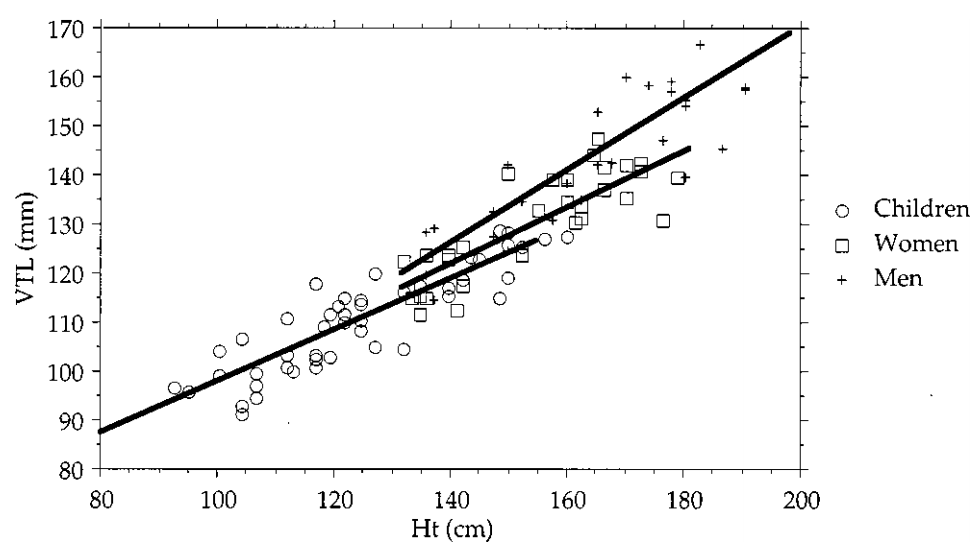
\includegraphics[width=.66\linewidth]{gfx/vocal-tract-size-sex.png}}
        \caption{Height (cm) versus vocal tract length (mm) \cite{Fitch1999}.}
        \label{fig:vocal-tract-morphology-sex}
\end{figure}

\begin{figure}[H]
        \myfloatalign
        {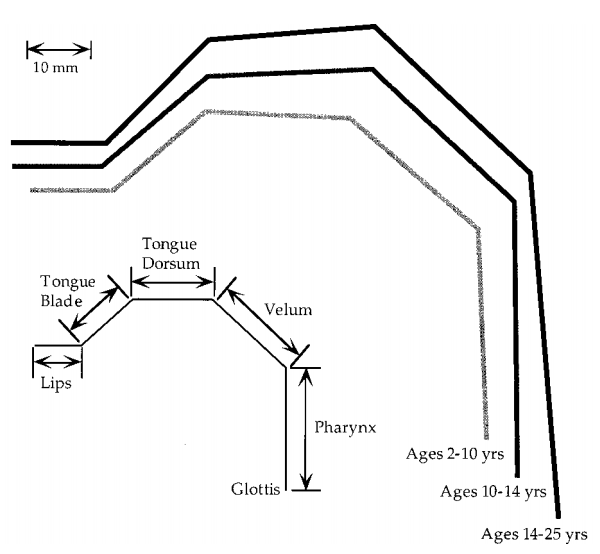
\includegraphics[width=.66\linewidth]{gfx/vocal-tract-size-gender.png}}
        \caption{Averaged vocal tract morphology \cite{Fitch1999}.}
        \label{fig:vocal-tract-morphology}
\end{figure}

As one can observe, men's vocal tract are longer than women's, followed and obviously children. These morphology differences 
affect the speech signal thorougly, specially in what concerns to the \ac{F0}. \ac{F0} can be defined as the 
lowest frequency in the signal counting from zero. \autoref{fig:f0-age-sex} compares the \ac{F0} values
between male and females considering aging.

\begin{figure}[!ht]
        \myfloatalign
        {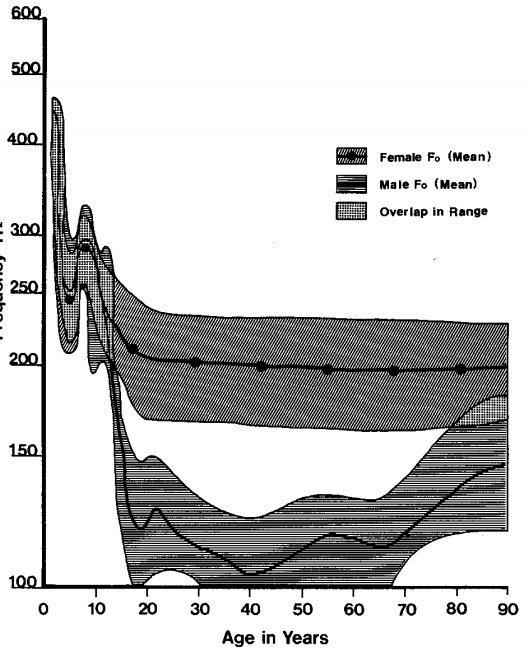
\includegraphics[width=.66\linewidth]{gfx/f0-age-sex.png}}
        \caption{F0 and pitch sigma versus age for males and females \cite{Brown1991}.}
        \label{fig:f0-age-sex}
\end{figure}

One can notice from \autoref{fig:f0-age-sex}, that no difference is found between male and female voice at a very young age. 
In fact, boys and girls have roughly the same \ac{F0} values. However, when they reach puberty, differences begin to appear. 
This period is commonly called the voice mutation or voice change, when the \ac{F0} for male voice has huge drop, while 
for female voice the drop is quite small. In terms of perception, this is period when the male voice lowers and geets deeper.

XXXXXXXXXXXXXXXXXXX EXTEND INTER-SPEAKER VARIABILITY
XXXXXXXXXXXXXXXXXXX DESCRIBE INTRA-SPEAKER VARIABILITY

But let's get back to \autoref{tab:comparison-human-mach}. It is interesting to notice that humans
performed better in all speech recognition tasks, but one: ``Clean speech based on trigram sentences''.
This one task consists of recognizing sentences which were randomly generated using the WSJ trigram language model. 
Therefore, humans had no advantage over machines in what concerns to syntactic or semantic knowledge. 
This result highlights one of the most important feature of human hearing, that is, we make a large use of syntactic, 
semantic and also pragmatic information in order to understand speech. While hearing do not take into account simply 
the acoustic signal, but the whole context. 

Language is a social tool, which aims at successfull interaction. When someone steps into a snack bar and orders 
an [\textipa{aIs"krim}], the vendor has no doubt that this sequence of phones refers to ``ice cream'' and not ``I scream'', 
albeit they are pronounced exactly the same. Although such sequence of phones might be ambiguous in the phonetic level,
it is not in higher linguistic levels, such as syntax (the verb ``order'' is usually followed by a noun), semantics 
(the object of order has to be something purchasable) and pragmatics (one does not buy his own shout!).


\subsection{HMM-based Speech Recognition} 
\ac{HMM} is the most widespread and successfull paradigm in \ac{ASR}. When \ac{HMM} were first applied
to speech recognition in the late $70$'s, they were completely revoluationary.
Up until recently \ac{DNN} seem to be next prominent paradigm in \ac{ASR}.
\ac{HMM} have been applied
to \ac{ASR} since the late $70$'s, and they have gathered the best results until recently.

A \ac{HMM} is a statistical Markov model in which the states are assumed to be hidden, i.e. they are
not directly visible, only the state's outputs are observable. Each state has a probability distribution 
over the possible output tokens, in such a way that output generated by the HMM states provides some information
about the hidden sequence of states which was traversed.

\subsection{Feature Extraction}

\paragraph{Preambulus}
Feature extraction is an importart part of speech recognition systems. The feacture extraction 
phase is responsible for identifying or enhancing the components of the signal that are relevant 
for recognizing speech sounds, while discarding or diminishing the effect of unuseful information, 
such as background noise. With respect to speech parameterization, \ac{MFCC} are definitely the
standard. \ac{MFCC} have been widely used in \ac{ASR} systems for almost three decades \cite{Davis1980}, 
they are present on the many important speech recognition toolkits, such as \ac{HTK}, Sphinx, \ac{RASR} and Kaldi.
Before we go into further details about these features it is interesting to give a little background 
about speech recording and coding.

Speech is recorded by using a microphone -- nothing new so far!
Despite the many types of available microphones (condenser, capacitor, pyezoeletric, laser, etc.) its design
remains basically the same as the carbon microphone invented by David Hughes two centuries ago \cite{Robjohns2010}.
A microphone is simply an acoustic-to-electric sensor, which converts variations in air pressure (that is, sound)
into an electrical signal. Microphones have a very thin membrane, called diaphragm, which vibrates when struck by 
sound waves.  When the diaphragm vibrates, it puts to move a sensitive capsule attached to it, 
that converts its movement into electrical pulses. Most of the current microphones are dynamic, which means 
that their capsule consist of  .... (XXX VER WIIPEDIA)

After capturing speech through a microphone, one usually wants to store it for later access. In order
to store speech digitally on a computer, a coding scheme is mandatory. In the literature, many coding schemes have
been proposed, such as linear PCM, $\mu$-law, A-law PCM, APCM, DPCM, DM, and ADPCM \cite{Huang2001}. The details of 
each type of speech coder is beyond the scope of this dissertation, the reader can 
find an description of each scheme in \citet{Huang2001} \citep{Huang2001} or \citet{Furui2001} \citep{Furui2001}. 
Following we will give a brief discussion of linear PCM, which is the standard way of storing audios in digital format. 

\ac{PCM} is a type of analog-to-digital conversion, which constitutes the basis of the WAV digital audio format, together
with other lossless formats such as AIF and AU.
\footnote{Other types of popular audio files which use lossy data compression, such as MP3, WMA, OGG or AAC (a format common to 
DivX videos) do not use PCM. Instead}. 
PCM coding is based on two properties: (i) a sampling rate of the audio and a (ii) bit depth. The sampling rate determines the
number of audio samples that are taken per second from the signal, in turn the bit depth is the number of bits 
of information in each audio sample. Both values must be constant and should be defined prior to recording (actually coding) an audio. 
The sampling and the bit depth are closely related to the audio quality, that is, the higher the sampling and the depth
the better the fidelity of the digital audio to the analog speech signal. Picture XXX presents an example of a linear PCM 
representation, at different sampling rates and bit depths, of an audio containing the utterance ``Speech recognition''.

Linear PCM assumes that the discrete signal $x[n]$ is bounded, that is,
\begin{equation}
|x[n]| \leq X_{max} 
\end{equation}
and that the quantization step $\Delta$ is uniform for all consecutive levels of $x_i$
\begin{equation}
x_i - x_{i-1} = \Delta
\end{equation}

Assuming a binary code, the number of levels which can be represented by PCM is $N=2^B$, where $B$ is the bit depth, this constitutes
the audio resolution. According to \citep{Huang2001}, speech could be represented in an intelligible way by using 7 bits, however, in 
practice, applications use values no lower than 11 bits to guarantee communication efficiency. For instance, CDs makes use of 16-bit 
linear PCM, whereas DVD-Audio and Blu-Ray discs can support up to 24-bit.

Although linear PCM files are able to carry all the necessary auditory information -- after all we are able to listen to them and
recognize the speech, the music or the noise recorded in them; they are not useful for speech recognition purposes. This occurs 
because, from the phonological point of view, very little can be said based on the waveform itself \citep{Shrawankar2010}.
Consider, for instance, the two combinations of 100 Hz, 200 Hz and 300 Hz sine waves, shown in \autoref{fig:complex-waves-pure-tones}, 
which differ only with respect to the relative timing.

\begin{figure}[!ht]
        \myfloatalign
        {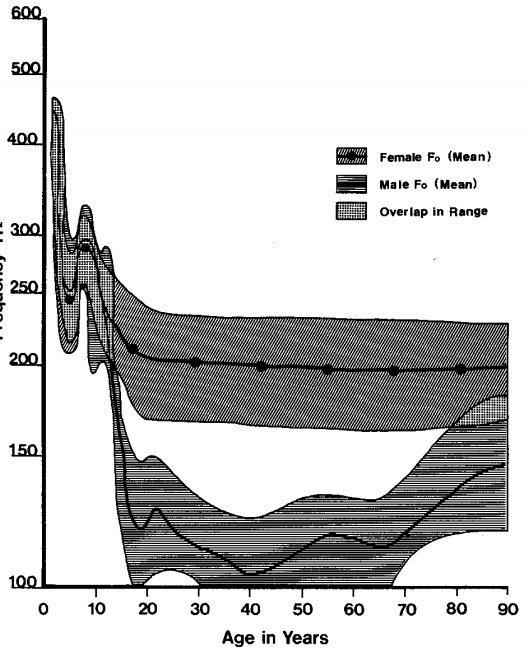
\includegraphics[width=.66\linewidth]{gfx/f0-age-sex.png}}
        \caption{Two complex waveforms generated by the same three pure tone 100 Hz, 200 Hz and 300 Hz sine waves, differing only 
        with respect to their relative timing \cite{Ladefoged1996}.}
        \label{fig:complex-waves-pure-tones}
\end{figure}
 
As one might notice, disregard of being composed by the same pure tones, the complex waves shown in 
\autoref{fig:complex-waves-pure-tones} are completely distinct from one another. This happens because the waveform is influenced
by phase shifts (also known as phase offsets). Therefore in-phase and out-of-phase waves (\autoref{fig:in-phase-waves} and
\autoref{fig:out-of-phase-waves}) are represented differently, and this adds too much variability to the waveform, in such way that
the signal waveform becomes unsuitable for human analysis and consequently for being used as a raw input in \ac{ASR} systems. 


\begin{figure}[!ht]
        \myfloatalign
        {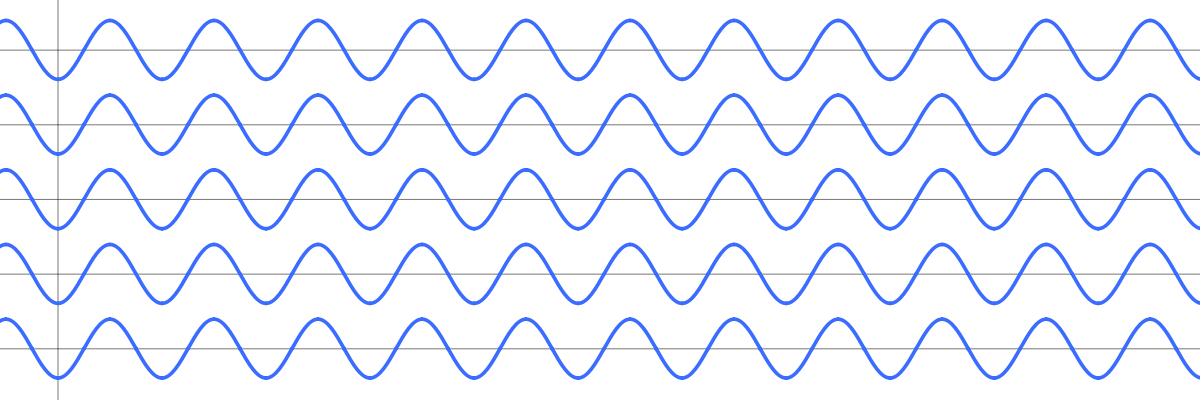
\includegraphics[width=.66\linewidth]{gfx/in-phase-waves.png}}
        \caption{Example of in-phase waves.}
        \label{fig:in-phase-waves}
\end{figure}

\begin{figure}[!ht]
        \myfloatalign
        {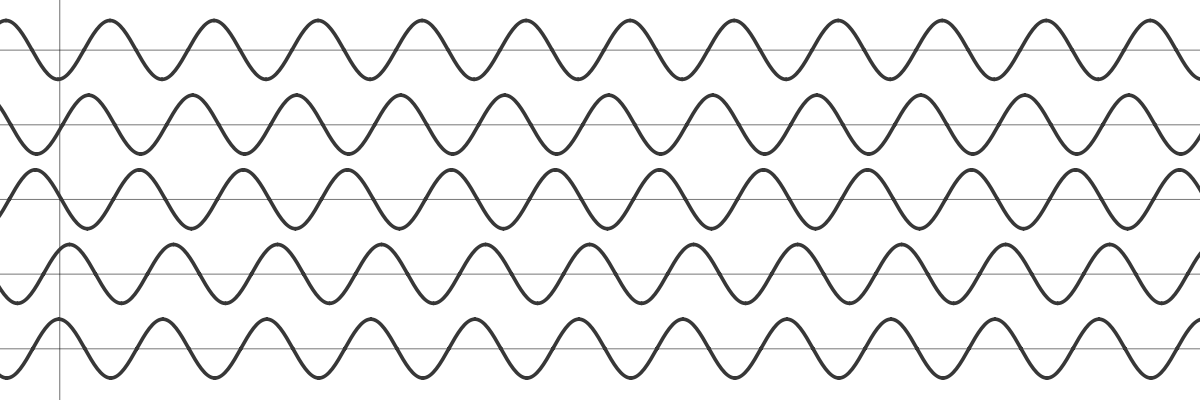
\includegraphics[width=.66\linewidth]{gfx/out-of-phase-waves.png}}
        \caption{Example of out-of-phase waves.}
        \label{fig:out-of-phase-waves}
\end{figure}

Another way of representing the audio information, which is more meaningful for human reading
or computer analysis is through short-term spectrum. Short-term spectra are obtained by applying
a Discrete Time Fourier transform to a windowed signal. At first, the signal is divided
into uniformly-spaced periods with a sliding window. For speech recognition, usually the window size is defined as 25 ms, 
with a frame shift of 10 ms, audio information is extracted every 10 ms with 15 ms of overlapping
among adjacent frames \cite{Huang2001}. \autoref{fig:audio-windowing} contains an example of a windowing process (in this case, 
with 50\% overlapping).

\begin{figure}[!ht]
        \myfloatalign
        {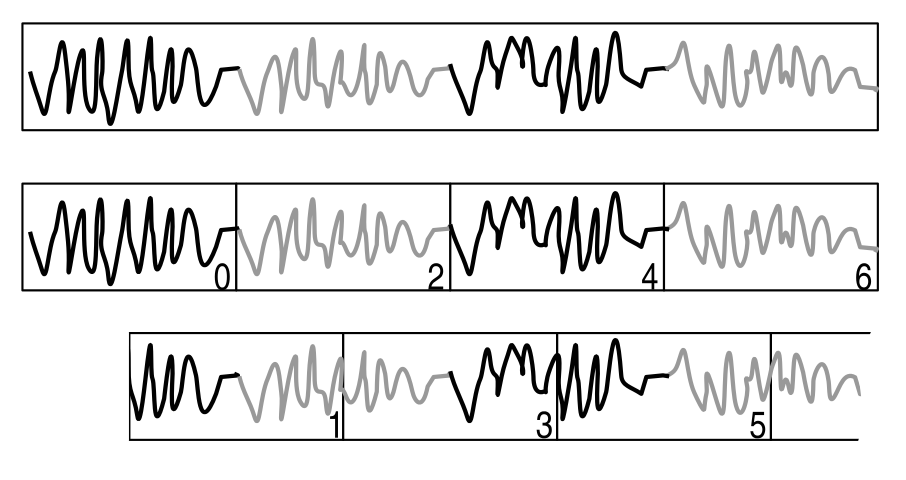
\includegraphics[width=.66\linewidth]{gfx/audio-windowing.png}}
        \caption{Illustration of an original audio recording (the upper waveform) divided into two
offset sequences of analysis windows (two lower waveforms) with 50\% overlapping frames \cite{McLoughlin2009}}
        \label{fig:audio-windowing}
\end{figure}

These windows values are based on two assuptions: (i) that within 25 ms the signal is stationary, i.e.
the phonatory system is not moving; (ii) that at least a period of each relevant speech frequency will 
be captured by this window
this windows, that is no relevant are 

After windowing the signal a Fourier transform is applied into each window so as to obtain
a series of frequency spectra, i.e. a series of representation of the signal in the frequency domain instead of the time domain. As can be noticed in \autoref{fig:audio-windowing}, since the frame shift is smaller than the window size, the windowing process extracts many redundant information. The intention for doing this will be made afterwards, when we give further details of the Fourier transform. Such transform is based on the Fourier theorem, which states that any periodic waveform can be approximated as closely as desired as the sum of a series of pure sine waves. In other words, the Fourier transform is able to analyse a short-term of the signal, containing a complex wave, and to output which are and what is the amplitude of the pure tones which form this complex wave.

Feature extraction must then be performed in stored audio files in order to extract relevant information from the waveform and discard redundant or unwanted signal characteristics. As already mentioned before, the two most traditional techniques for speech feature extraction, over the past decades, have been the \ac{MFCC} \cite{Davis1980} and the \ac{PLP} \cite{Hermansky1990}. Both parameterization methods are based on the short-term spectrum of speech. For speech recognition purposes, \ac{MFCC} features usually show better performance when compared to \ac{PLP}, for this reason in this thesis we are only going to present \ac{MFCC} features \cite{Muller2001, Mporas2007}.

\subsection{MFCC Features}

\ac{MFCC} is a type of speech parameterization is the result of a cosine transform of the logarithm of the short-term energy spectrum expressed over a mel scale \cite{Davis1980}. \ac{MFCC} features tries to reduce the feature dimensionality of a sound Fourier spectrum, by applying some concepts of Psychoacoustics and Psychophysics in order to the extract a vector with relevant values from the spectrum. The aim is to represent speech data in a compressed format, by eliminating information which are not pertinent to the phonetic analysis and to enhance the aspects of the signal which contribute to the detection of phonetic differences \cite{Davis1980}.

From Psychoacoustics, \ac{MFCC}s use the notion that humans do not perceive frequency through a linear scale, but through a scale which resembles to be linear-spaced in frequencies below 1000 Hz and logarithmic in frequecies above 1000 Hz\footnote{This is not entirely true. As shown by \citet{Umesh1999}~\cite{Umesh1999}, in fact, there are no two distinguishable regions in terms of statistical significance. But the idea that we perceive low frequencies better than high ones still hold.}, the so-called mel scale (named after \emph{mel}ody). The scale is based on experiments with simple tones in which individuals are required to separat frequency values into four equal intervals or to adjust the frequency of a stimulus to be half as high as another reference tone \cite{Huang2001}. The reference point between mel scale and a linear frequency scale is 1000 mels, which correspond to a 1000 Hz tone, 40 dB above the absolute threshold of hearing. Since it was first introduced by \citet{Stevens1937}~\cite{Stevens1937}, the scale has been revisited many times \cite{Umesh1999}, but a common formulation, according to \citet{Huang2001}~\cite{Huang2001} is:
\begin{equation}
 M(f) = 1125*ln(1 + f / 700)
\end{equation}
where $f$ is the input frequency in Hz. The scale is plotted \autoref{fig:mel-scale}.
\begin{figure}[!ht]
        \myfloatalign
        {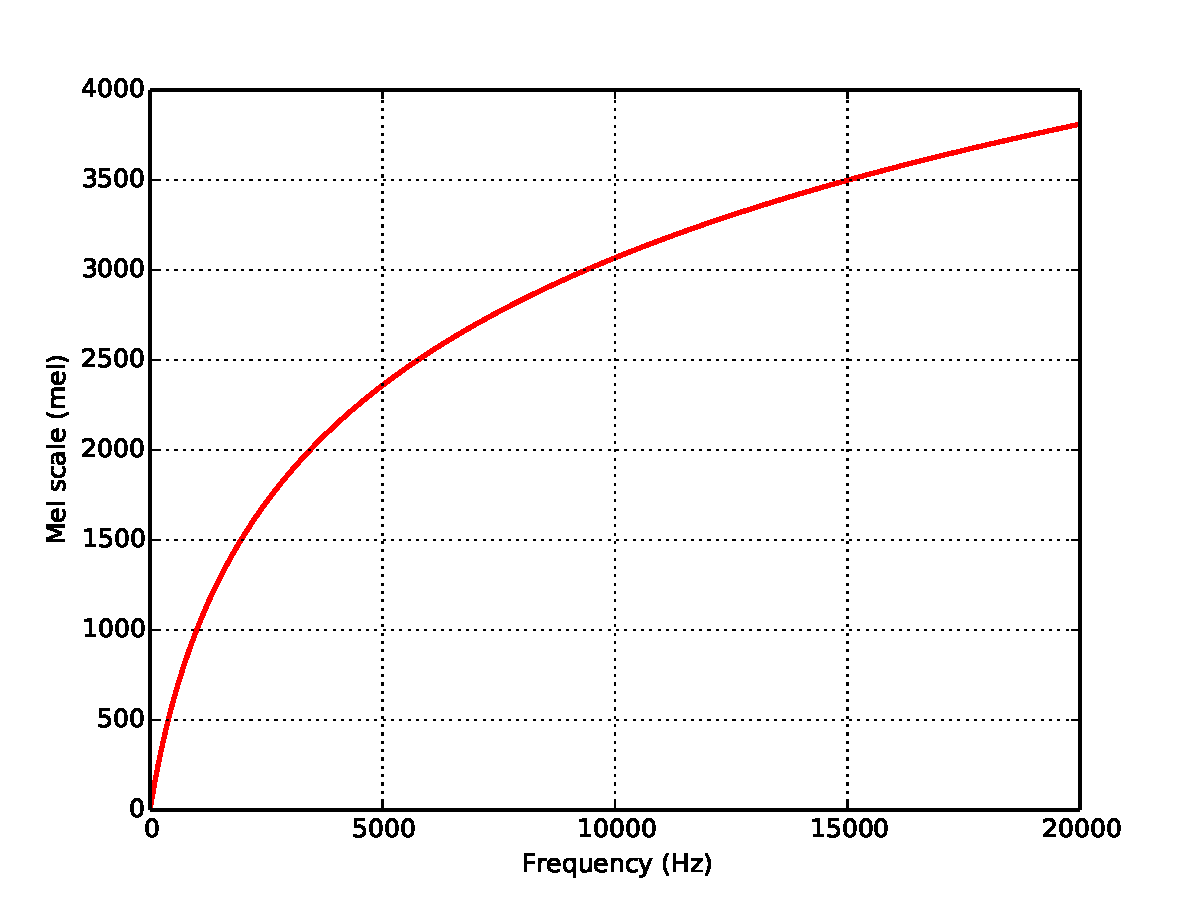
\includegraphics[width=1.\linewidth]{gfx/mel-scale.pdf}}
        \caption{Mel scale versus a linear frequency scale.}\label{fig:mel-scale}
\end{figure}

and also of the physics of speech, such as the fact that human like the these systems often have well defined overtones that are harmonic -- which is why the MFCCs use the FFT of the FFT)


\subsection{Dealing with Noisy Data}

One of the central problems in \ac{ASR} is how to deal with noisy audio data. It is long known that the performance of 
speech recognition systems greatly degrate when the environmental or the recording conditions are not controlled, 
thus allowing unwanted residual sounds to appear in the signal. In acoustics, any type of sound that is not the one
you are willing to analyze is considered noise. As a result from this, in speech recognition, the hiss of a fan, 
the buzz that a computer cooler makes, car horns on the street and so on are all regarded as noise. Even someone's voice
can be regarded as noise. Consider, for instance, that you are trying to recognize John's speech in an application, 
however Mary is close to him talking on the phone, to the extent that traces of her voice are added to the signal. In this
scenario, Mary's voice is actually noisy data, since it is undesirable for the given purpose. 

\subsection{Types of Speech Recognition Systems} 
Errem omnium ea per, pro \ac{UML} congue populo ornatus cu, ex qui
dicant nemore melius. No pri diam iriure euismod. Graecis eleifend
appellantur quo id. Id corpora inimicus nam, facer nonummy ne pro,
kasd repudiandae ei mei. Mea menandri mediocrem dissentiet cu, ex
nominati imperdiet nec, sea odio duis vocent ei. Tempor everti
appareat cu ius, ridens audiam an qui, aliquid admodum conceptam ne
qui. Vis ea melius nostrum, mel alienum euripidis eu.

\subsection{The Architecture of a Large Vocabulary Continuous Speech Recognition System} 
Non vices medical da. Se qui peano distinguer demonstrate, personas
internet in nos. Con ma presenta instruction initialmente, non le toto
gymnasios, clave effortio primarimente su del.


%*****************************************
%*****************************************
%*****************************************
%*****************************************
%*****************************************